%%%%%%%%%%%%%%%%%%%%%%%%%%%%%%%%%%%%%%%%%%%%%%%%%%%%%%%%%%%%%%%%%%%%%%%%%%%%%%%%
%	TRABAJO: Proyecto Integrador
%		Titulo: 	Desarrollo de IP cores con procesamiento de Redes de Petri 	
%					Temporales para sistemas multicore en FPGA					
%		Autores:	Juli�n Nonino												%					Carlos Renzo Pisetta										%		Director:	Orlando Micolini											
%%%%%%%%%%%%%%%%%%%%%%%%%%%%%%%%%%%%%%%%%%%%%%%%%%%%%%%%%%%%%%%%%%%%%%%%%%%%%%%%

% Path im�genes: ./desarrollo/diseno_implementacion/img
% Nombre predeterminado im�genes: disenoxx
%	xx es el numero de imagen

\lstset
{	language=Verilog,               % the language of the code
	basicstyle=\footnotesize,       % the size of the fonts that are used for the code
	numbers=left,                   % where to put the line-numbers
	numberstyle=\tiny\color{gray},  % the style that is used for the line-numbers
	stepnumber=1,                   % the step between two line-numbers. If it's 1, each line 
                       				% will be numbered
	numbersep=5pt,                  % how far the line-numbers are from the code
	backgroundcolor=\color{white},  % choose the background color. You must add \usepackage{color}
	showspaces=false,               % show spaces adding particular underscores
	showstringspaces=false,         % underline spaces within strings
	showtabs=false,                 % show tabs within strings adding particular underscores
	frame=none,                 	% adds a frame around the code
	rulecolor=\color{white},        % if not set, the frame-color may be changed on line-breaks within not-black text (e.g. comments (green here))
	tabsize=2,                      % sets default tabsize to 2 spaces
	captionpos=b,                   % sets the caption-position to bottom
	breaklines=true,                % sets automatic line breaking
	breakatwhitespace=false,        % sets if automatic breaks should only happen at whitespace
	%title=\lstname,                % show the filename of files included with \lstinputlisting;
		                            % also try caption instead of title
	keywordstyle=\color{blue},      % keyword style
  	commentstyle=\color{dkgreen},   % comment style
  	stringstyle=\color{mauve},      % string literal style
  	escapeinside={\%*}{*)},         % if you want to add LaTeX within your code
  	morekeywords={*,...},           % if you want to add more keywords to the set
  	deletekeywords={...}            % if you want to delete keywords from the given language
}

\chapter{Dise�o e Implementaci�n}
	\label{chap:chap_diseno_implementacion}

	En esta secci�n se describir� la implementaci�n de un \textbf{\emph{procesador de Petri}}, un \emph{IP-Core} que resuelve \emph{Redes de Petri con Arcos Inhibidores} en los que se restringe el disparo de transiciones y \emph{Redes de Petri Temporales} donde se introduce el tiempo como condici�n de ejecuci�n. En la primera secci�n de este capitulo, se presentar� la arquitectura general del sistema. En las secciones siguientes se explicar� el dise�o y la implementaci�n del procesador de Redes de Petri dividido en dos partes. En la primera parte, se realizo una refactorizaci�n del trabajo descripto en el trabajo \cite{galliapereyra}. Esta refactorizaci�n se realiz� para utilizar Verilog como HDL en lugar del lenguaje VHDL, esto se realiz� por razones de claridad, y adem�s, para permitir una implementaci�n parametrizable que sea mas apta para el agregado de la funcionalidad de procesamiento de Redes de Petri Temporales. En la segunda etapa del proyecto, se dise�� e implement� un IP core para el procesamiento de \textbf{\emph{Redes de Petri con Tiempo}} y otro para la resoluci�n de \textbf{\emph{Redes de Petri Temporizadas}}.
	
	% Arquitectura general del sistema
		%%%%%%%%%%%%%%%%%%%%%%%%%%%%%%%%%%%%%%%%%%%%%%%%%%%%%%%%%%%%%%%%%%%%%%%%%%%%%%%%
%	TRABAJO: Proyecto Integrador
%		Titulo: 	Desarrollo de IP cores con procesamiento de Redes de Petri 	
%					Temporales para sistemas multicore en FPGA					
%		Autores:	Juli�n Nonino												%					Carlos Renzo Pisetta										%		Director:	Orlando Micolini											
%%%%%%%%%%%%%%%%%%%%%%%%%%%%%%%%%%%%%%%%%%%%%%%%%%%%%%%%%%%%%%%%%%%%%%%%%%%%%%%%

% Path im�genes: ./desarrollo/diseno_implementacion/img
% Nombre predeterminado im�genes: disenoxx
%	xx es el numero de imagen

\section{Arquitectura general del sistema}
	\label{sec:arquitectura_general}

	Al comenzar el trabajo, se creo un esquema para describir la ubicaci�n y la conexi�n del procesador de Petri en un sistema multicore.
	\begin{figure}[ht]
		\centering
		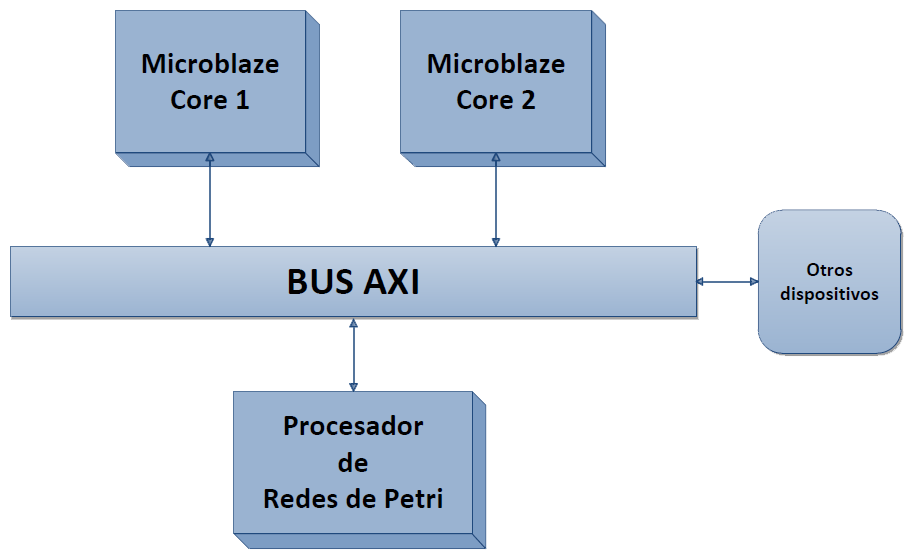
\includegraphics[width=1\linewidth,keepaspectratio]{./desarrollo/diseno_implementacion/img/diseno01}
		\caption{Arquitectura general del sistema}
		\label{fig:diseno01}
	\end{figure}
	
	En el diagrama de la \ref{fig:diseno01}, se observa como esta ubicado el procesador de Petri dentro del sistema. Existen dos cores MicroBlaze de Xilinx que a trav�s del BUS AXI se comunicaran con el procesador de Petri para sincronizarse. Se plante� un sistema con dos procesadores ya que este es el m�nimo numero de cores para que el sistema sea multicore. El procesador de Redes de Petri se encuentra conectado al bus AXI independientemente de los otros procesadores del sistema porque de esta forma, la �nica limitaci�n en el acceso al procesador de Redes de Petri ser�a el bus.
	
	% Procesador de Petri (primera etapa)
		%%%%%%%%%%%%%%%%%%%%%%%%%%%%%%%%%%%%%%%%%%%%%%%%%%%%%%%%%%%%%%%%%%%%%%%%%%%%%%%%
%	TRABAJO: Proyecto Integrador
%		Titulo: 	Desarrollo de IP cores con procesamiento de Redes de Petri 	
%					Temporales para sistemas multicore en FPGA					
%		Autores:	Juli�n Nonino												%					Carlos Renzo Pisetta										%		Director:	Orlando Micolini											
%%%%%%%%%%%%%%%%%%%%%%%%%%%%%%%%%%%%%%%%%%%%%%%%%%%%%%%%%%%%%%%%%%%%%%%%%%%%%%%%

% Path im�genes: ./desarrollo/diseno_implementacion/img
% Nombre predeterminado im�genes: disenoxx
%	xx es el numero de imagen

\section{Procesador de Petri (primera etapa)}
	\label{sec:proc_petri_primera_etapa}

	Como se dijo, en esta primera etapa se realiz� una refactorizaci�n de un trabajo anterior. Para ello, se dise�o nuevamente el sistema generando una arquitectura mas modular que permita la adici�n de funcionalidad nueva de manera sencilla y clara. Adem�s, se dise�o pensando en nuevas caracter�sticas.
	
	\subsection{Requerimientos}
		
		Los requerimientos para esta etapa fueron:
		\begin{enumerate}
			\item: Refactorizar el trabajo descripto en \cite{galliapereyra} generando una arquitectura modularizada en Verilog.
			\item: Implementar el procesamiento con plazas acotadas o limitadas.
			\item: Generar la posibilidad de que se disparen transiciones de manera autom�tica al estar sensibilizadas, sin necesidad de esperar un pedido de disparo explicito.
		\end{enumerate}
	
	\subsection{Arquitectura}
		
		A continuaci�n presentamos la arquitectura del primer procesador de Redes de Petri, el cual est� basado en el algoritmo de ejecuci�n de Redes de Petri (descripto en la secci�n \ref{subsec:redes_con_tiempo}) implementado. Y luego, se describe todas sus funcionalidades e interrelaci�n.
		\newpage
			\begin{figure}[ht]
				\centering
				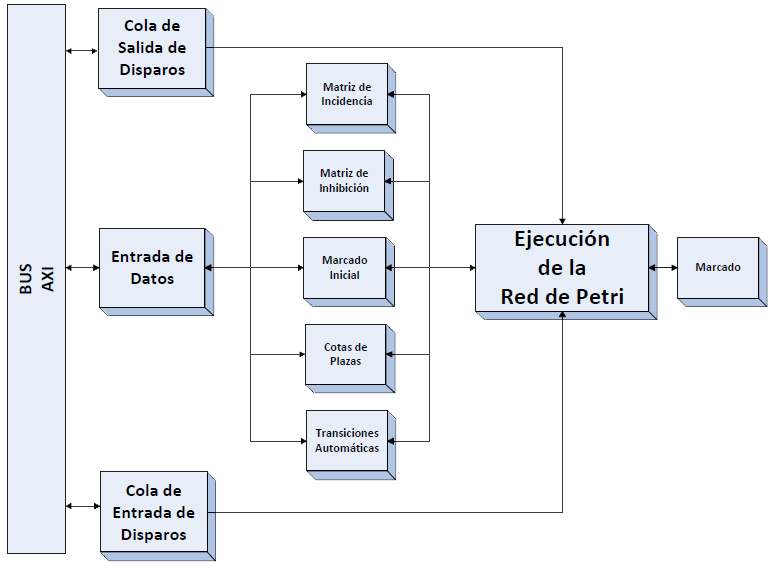
\includegraphics[width=1\linewidth,keepaspectratio]{./desarrollo/diseno_implementacion/img/diseno02}
				\caption{Arquitectura del procesador de Redes de Petri (Primera Parte)}
				\label{fig:diseno02}
			\end{figure}
		
		\subsubsection{Matriz de Incidencia}
			
			La matriz de incidencia, como ya se vio, es una matriz que tiene como cantidad de filas el n�mero de plazas y como cantidad de columnas el n�mero de transiciones. Cada elemento de esta matriz es un n�mero entero con signo.
			\begin{lstlisting}
//Parametros
	parameter cant_plazas			= 15;
	parameter cant_transiciones		= 10;
	parameter tamano_de_elementos	= 6;

//Matriz de incidencia
	reg signed [tamano_de_elementos-1:0] matriz_incidencia [cant_plazas-1:0] [cant_transiciones-1:0];
\end{lstlisting}
		
		\subsubsection{Matriz de inhibici�n}
			
			La matriz de inhibici�n, se declar� de manera similar a la matriz de incidencia. La �nica diferencia con la anterior es que �sta es una matriz binaria. Por lo tanto, cada elemento de esta matriz es de \textbf{un bit}.		
			\begin{lstlisting}
//Matriz de Arcos Inhibidores
	reg matriz_inhibicion [cant_plazas-1:0] [cant_transiciones-1:0];
			\end{lstlisting}

		\subsubsection{Marcado inicial y marcado}
		
			Dado que en Verilog una variable no puede ser modificada en m�s de un \emph{always}, existen dos vectores para almacenar el marcado de la red. Uno llamado \textbf{\emph{marcado inicial}} que es modificado durante la carga de datos. Y, otro llamado \textbf{\emph{marcado}} que es el que almacena el marcado actual de la red y que al comienzo toma el valor que tiene el vector \textbf{\emph{marcado inicial}}.
			\begin{lstlisting}
//Marcado
	reg [tamano_de_elementos-1:0] marcado [cant_plazas-1:0];
	reg [tamano_de_elementos-1:0] marcado_inicial [cant_plazas-1:0];	
			\end{lstlisting}
		
		\subsubsection{Cotas de plazas}
		
			Las cotas en las plazas, se implementan mediante un vector cuya cantidad de elementos es el n�mero de plazas. En realidad, como se esta implementado hardware, todas las plazas est�n limitadas al tama�o de elementos del vector de marcado. Por lo tanto, el vector de cotas, tendr� como tama�o de elementos el mismo que tiene el vector de marcado pudiendo limitar la cantidad de tokens en una plaza desde cero hasta este valor.
			\begin{lstlisting}
//Plazas acotadas
	reg [tamano_de_elementos-2:0] cotas_plazas [cant_plazas-1:0];
			\end{lstlisting}
		
		\subsubsection{Transiciones autom�ticas}
		
			Es un vector binario cuya cantidad de elementos es el n�mero de transiciones. Un \emph{uno} en alg�n elemento indica que la transici�n representada por el mismo es autom�tica y no debe esperar hasta que se solicite su disparo para dispararse, es decir, al momento que se sensibiliza se dispara.		
			\begin{lstlisting}
//Transiciones automaticas
	reg [cant_transiciones-1:0] transiciones_automaticas;
			\end{lstlisting}
		
		\subsubsection{Colas de disparos}
		
			Las colas de disparos son dos, una, para los disparos de entrada que esperan por ser ejecutados en cuanto la red lo permita. Y la otra, para los disparos de salida que ya han sido ejecutados y esperan a que el proceso que solicit� su ejecuci�n los extraiga. La implementaci�n de estas colas se realiza con un contador por cada transici�n que indica cuantos disparos pendientes o ya ejecutados existen para dicha transici�n. Adem�s, existe un vector binario que indica si la cola de una determina transici�n esta vac�a o tiene alg�n valor. Esta implementaci�n obedece a la necesidad de insertar o extraer los disparos en un ciclo de reloj y adem�s, poder contemplar todas las solicitudes de disparos de las distintas transiciones en paralelo.
				\begin{figure}[H]
					\centering
					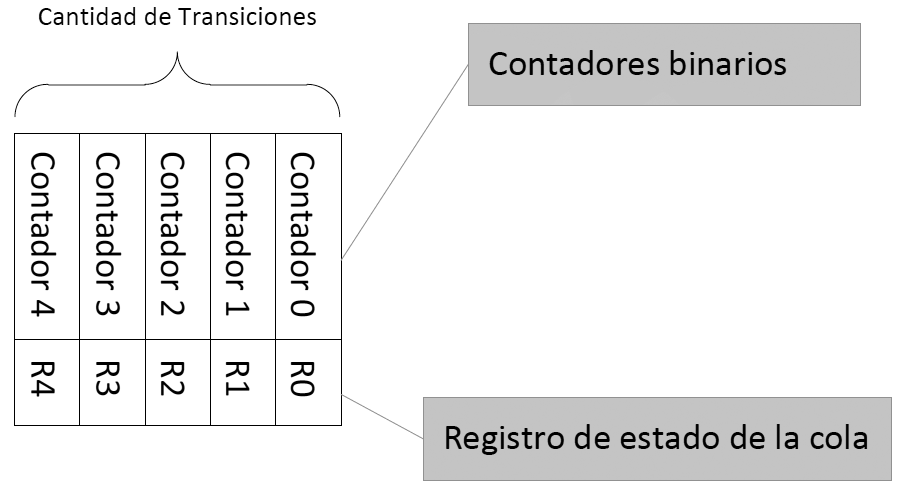
\includegraphics[width=1\linewidth,keepaspectratio]{./desarrollo/diseno_implementacion/img/diseno03}
					\caption{Esquema de las colas de disparos}
					\label{fig:diseno03}
				\end{figure}
			Cada una de las posiciones del vector de estado de la cola indican si esta vac�o o no. Esto se hace de la siguiente manera:
				\begin{figure}[H]
					\centering
					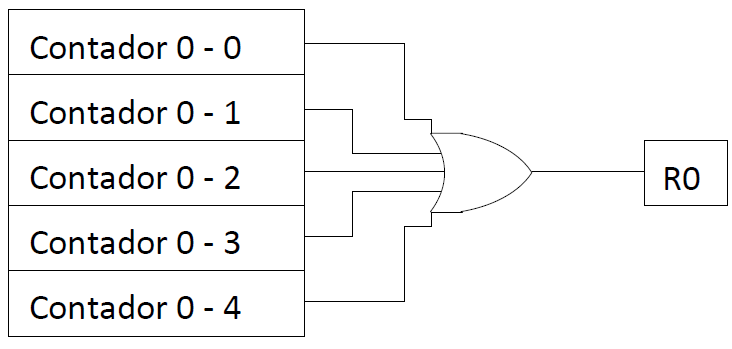
\includegraphics[width=1\linewidth,keepaspectratio]{./desarrollo/diseno_implementacion/img/diseno04}
					\caption{Registro que indica si las colas de disparos est�n vac�as o no}
					\label{fig:diseno04}
				\end{figure}
			Un uno es este vector indica que la cola contiene al menos un elemento. Adem�s, se implementa otro registro de estado que indica si la cola esta llena o no. Este registro se implement� de la siguiente manera. Un uno es este vector indica que la cola esta llena y no puede recibir mas elementos.		
				\begin{figure}[H]
					\centering
					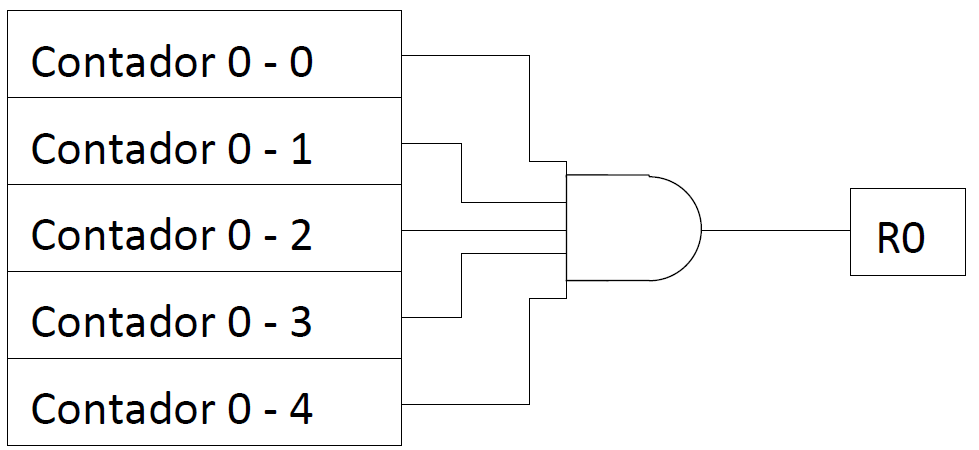
\includegraphics[width=1\linewidth,keepaspectratio]{./desarrollo/diseno_implementacion/img/diseno05}
					\caption{Registro que indica si las colas de disparos est�n llenas o no}
					\label{fig:diseno05}
				\end{figure}
			La implementaci�n de estas colas se realizo en un modulo de Verilog que luego fue instanciado dos veces. Una vez, para la cola de disparos de entrada y otra, para la cola de salida.
			\begin{lstlisting}
/****************************COLA DE ENTRADA DE DISPAROS**********************/
		
	reg [cant_transiciones-1:0] disparo_entrada_incrementa;
	reg [cant_transiciones-1:0] disparo_entrada_decrementa;
	reg [tamano_cola-1:0] counter_cola_disparos_entrada [cant_transiciones-1:0]/* synthesis syn_keep = 1 */;
	integer index_entrada;
	always @(posedge Bus2IP_Clk)
	begin
		if(Bus2IP_Resetn==1'b0)
		begin
			for (index_entrada=0 ; index_entrada<cant_transiciones ; index_entrada=index_entrada+1)
			begin
				counter_cola_disparos_entrada[index_entrada]<={tamano_cola{1'b0}};
			end
		end
		else	
			for (index_entrada=0 ; index_entrada<cant_transiciones ; index_entrada=index_entrada+1)
			begin
				//Incremento cola entrada
					if ({disparo_entrada_incrementa[index_entrada] , disparo_entrada_decrementa[index_entrada]} == 2'b10) //Debe incrementar 
					begin
						counter_cola_disparos_entrada[index_entrada] <= counter_cola_disparos_entrada[index_entrada] + 1'b1;
					end //FIN if(disparo_entrante[index_entrada] == 1'b1)
				//Decremento cola entrada	
					else if ({disparo_entrada_incrementa[index_entrada] , disparo_entrada_decrementa[index_entrada]} == 2'b01) //Debe decrementar  
					begin
						counter_cola_disparos_entrada[index_entrada] <= counter_cola_disparos_entrada[index_entrada] - 1'b1;// {tamano_cola{1'b1}};
					end //FIN if(disparo_dec_entrante[index_entrada] == 1'b1)
				//Otras opciones
					else
					begin
						counter_cola_disparos_entrada[index_entrada] <= counter_cola_disparos_entrada[index_entrada];
					end
			end //FIN for (index_entrada=0 ; index_entrada<cant_transiciones ; index_entrada=index_entrada+1)
	end //FIN always

/****************************COLA DE SALIDA DE DISPAROS**********************/
	reg [tamano_cola-1:0] counter_cola_disparos_salida [cant_transiciones-1:0]/* synthesis syn_keep = 1 */;
	reg [cant_transiciones-1:0] disparo_salida_incrementa;
	reg [cant_transiciones-1:0] disparo_salida_decrementa;
	integer index_salida;
	always @(posedge Bus2IP_Clk)
	begin
		if(Bus2IP_Resetn==1'b0)
		begin
			for (index_salida=0 ; index_salida<cant_transiciones ; index_salida=index_salida+1)
			begin
				counter_cola_disparos_salida[index_salida]<={tamano_cola{1'b0}};
			end
		end
		else	
			for (index_salida=0 ; index_salida<cant_transiciones ; index_salida=index_salida+1)
			begin
				//Incremento cola salida
					if ({disparo_salida_incrementa[index_salida] , disparo_salida_decrementa[index_salida]} == 2'b10) //Debe incrementar 
					begin
						counter_cola_disparos_salida[index_salida] <= counter_cola_disparos_salida[index_salida] + 1'b1;
					end //FIN if(disparo_salida_decrementa[index_salida] == 1'b1)
				//Decremento cola salida	
					else if ({disparo_salida_incrementa[index_salida] , disparo_salida_decrementa[index_salida]} == 2'b01) //Debe decrementar 
					begin
						counter_cola_disparos_salida[index_salida] <= counter_cola_disparos_salida[index_salida] - 1'b1;//{tamano_cola{1'b1}};
					end //FIN if(disparo_salida_decrementa[index_salida] == 1'b1)
				//Otras opciones
					else 
					begin
						counter_cola_disparos_salida[index_salida] <= counter_cola_disparos_salida[index_salida];
					end
			end //FIN for (index_salida=0 ; index_salida<cant_transiciones ; index_salida=index_salida+1)
	end //FIN always
			\end{lstlisting}
		
		\subsubsection{Ejecuci�n de la Red de Petri}
			
			El modulo ejecuci�n de la Red de Petri es el encargado de resolver la ecuaci�n de estado (\ref{eq:ecuacion_estado_uno}) de la red con los disparos que est�n pendientes y realizar la actualizaci�n del marcado en caso de ser necesario. Su funcionamiento ser� explicado en detalle en el apartado \ref{subsec:func_proc_petri}.
		
		\subsubsection{Entrada de datos}
			
			Este modulo es el encargado de cargar todos los datos con los cuales debe operar el Procesador de Redes de Petri para ejecutar la red. Su funcionamiento ser� explicado con detalle en el titulo \ref{subsec:func_proc_petri}.
				
	\subsection{Funcionamiento del procesador de Redes de Petri}
		\label{subsec:func_proc_petri}
		
		En esta secci�n, se presentar�n los diagramas desarrollados con el fin de explicar el funcionamiento del procesador de Redes de Petri mostrando la implementaci�n en Verilog de cada uno de los componentes.
		
		\subsubsection{Carga de datos}
			
			El modulo de carga de datos es el primero que debe entrar en acci�n al utilizar el procesador de Redes de Petri, a trav�s de �l se carga la matriz de incidencia, la matriz de inhibici�n, el marcado inicial, el vector de cotas de plazas y el vector de transiciones autom�ticas.
				\begin{figure}[H]
					\centering
					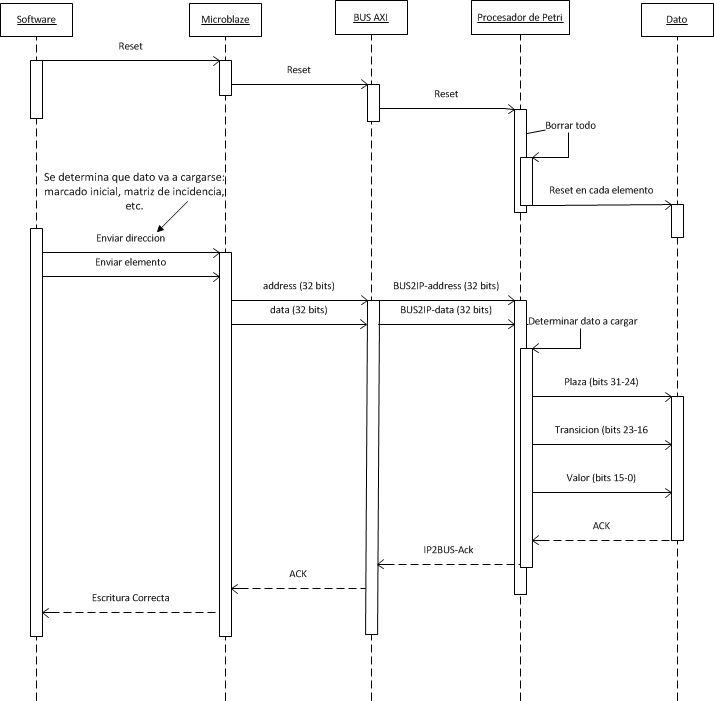
\includegraphics[width=1\linewidth,keepaspectratio]{./desarrollo/diseno_implementacion/img/diseno06}
					\caption{Diagrama de secuencia proceso de carga de datos}
					\label{fig:diseno06}
				\end{figure}
			El software, que se ejecuta en un procesador MicroBlaze desea cargar datos en alguno de los valores representativos de una Red de Petri (matriz de incidencia, marcado inicial, etc.) para programarlo o reprogramarlo. El proceso de carga de datos, se diagram� en la Figura \ref{fig:diseno06} dividido en dos partes. Una secuencia inicial de reset y una secuencia de carga de los elementos que se requieran para programar el funcionamiento del procesador de Petri.
			\\

			\textbf{Secuencia de reset de datos}
				
				La secuencia de reset, se compone de las siguientes etapas.
				\begin{enumerate}
				  	\item El software indica que el procesador MicroBlaze debe ejecutar un reset sobre el procesador de Petri.
				  	\item El procesador MicroBlaze env�a esta orden al procesador de Redes de Petri a trav�s de BUS AXI.
				  	\item El procesador de Redes de Petri procede a borrar todos los valores almacenados poniendo a cero todos los elementos de cada uno de ellos (marcado inicial, matriz de incidencia, etc.)
				\end{enumerate}
		
		
			\textbf{Secuencia de carga de un elemento}	
				
				Se debe aclarar que para la carga de un valor se utiliza una palabra especial de 32 bits, definida de la siguiente manera:
					\begin{figure}[H]
						\centering
						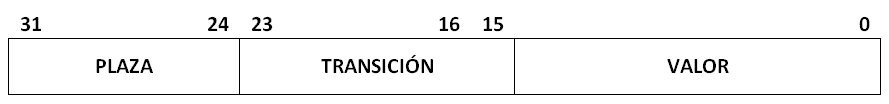
\includegraphics[width=1\linewidth,keepaspectratio]{./desarrollo/diseno_implementacion/img/diseno07}
						\caption{Palabra para la carga de datos en el procesador de Petri}
						\label{fig:diseno07}
					\end{figure}
				
				Esta palabra especial, reserva ocho bits para identificar las plazas y ocho bits para identificar la transici�n. Esto permite una Red de Petri con un m�ximo de 256 plazas y 256 transiciones que se considera tama�o suficiente para la mayor�a de los problemas a resolver. Los restantes 16 bits, identifican el valor que debe ir en el elemento indicado por el n�mero de plaza y por el n�mero de transici�n. Por ejemplo, si se esta cargando la matriz de incidencia y se env�a la siguiente palabra 00000101 00000011 1111111111111101, se cargara en el elemento de la fila 5 y columna 3 el valor -3. Si se carga por ejemplo el marcado inicial, para indicar que la plaza 7 tiene dos tokens al inicio se debe enviar la siguiente palabra 00000111 XXXXXXXX 0000000000000010. Aclarado esto, se explicar� la secuencia de carga.
				
				\begin{enumerate}
				  	\item El software decide cargar un valor, por lo tanto, mediante una direcci�n y un elemento le indica al MicroBlaze lo que debe ejecutar.
				  	\item El MicroBlaze, env�a a trav�s del BUS AXI la palabra de direcci�n y la palabra de dato (address y data).
				  	\item El procesador de Petri identifica que dato se desea cargar mediante la palabra address (si es matriz de incidencia, marcado inicial, etc.). Luego, interpretando la palabra de datos como se mencion� anteriormente, determina que valor se desea escribir y en que posici�n hacerlo.
				  	\item En cada escritura correcta se env�a un ACK para que el software sepa que la operaci�n se realizo con �xito.   
				\end{enumerate}		

		\subsubsection{Llegada de un nuevo disparo por ejecutar}
			
			Cuando llega un nuevo disparo, se utiliza la misma palabra definida en la Figura \ref{fig:diseno07}. Adem�s el procedimiento es bastante similar solo que debe verificarse que la cola de entrada de disparos correspondientes no se encuentre llena.		
				\begin{figure}[H]
					\centering
					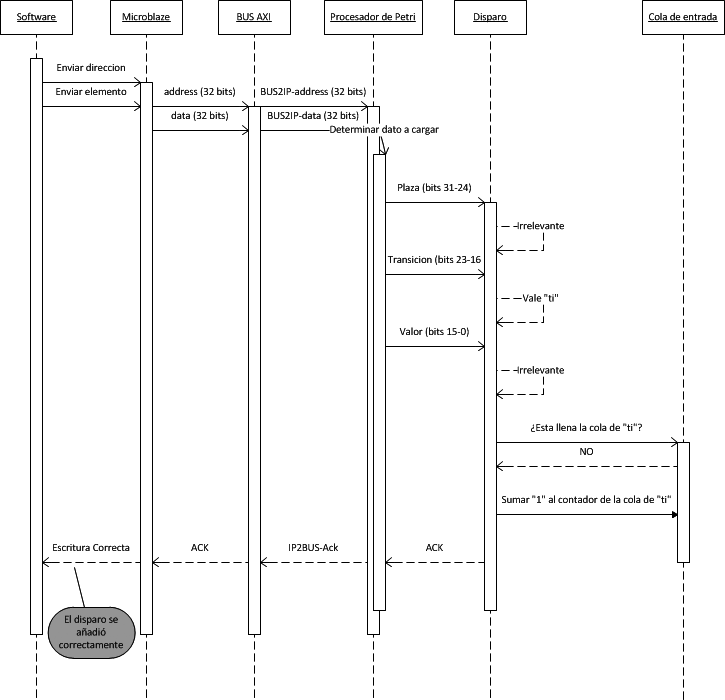
\includegraphics[width=1\linewidth,keepaspectratio]{./desarrollo/diseno_implementacion/img/diseno08}
					\caption{Diagrama de secuencia del ingreso de un nuevo disparo}
					\label{fig:diseno08}
				\end{figure}
			En la secuencia anterior, se observa que el proceso de env�o de un nuevo disparo para que sea ejecutado por el procesador de Redes de Petri es similar al proceso de carga de datos. La diferencia radica en la consulta a la cola acerca de si esta llena o no. Si la cola no esta llena, el disparo es a�adido a la cola y queda a la espera de ser ejecutado. En la Figura \ref{fig:diseno08} no se muestra el caso de que la cola si este llena. Lo que sucede en este caso no se a�ade el disparo a la cola y no se env�a el ACK. De esta manera, el software sabe que la escritura no fue correcta, es decir, el disparo no fue a�adido a la cola.
			
		\subsubsection{Algoritmo de ejecuci�n de Redes de Petri}		
			
			El algoritmo de ejecuci�n de Redes de Petri consiste en detectar los disparos que sean posibles de ser ejecutados y en caso de serlo, resolver la ecuaci�n de estado de la red para lograr un nuevo marcado de la misma. Recordado, la ecuaci�n de estado de una Red de Petri con Arcos Inhibidores \ref{eq:estado_petri_arcos_inhibidores}, tiene la siguiente forma:
				\begin{equation}
					m_{i+1}=m_i+I�[\delta\; and\; f_H(m_i,\;\delta)]
				\end{equation}
			
			La Figura \ref{fig:diseno09} ilustra como se ha implementado la resoluci�n de la ecuaci�n anterior determinando que transiciones est�n sensibilizadas y de acuerdo con los disparos en las colas o aquellas transiciones que son autom�ticas. 
				\begin{figure}[ht]
					\centering
					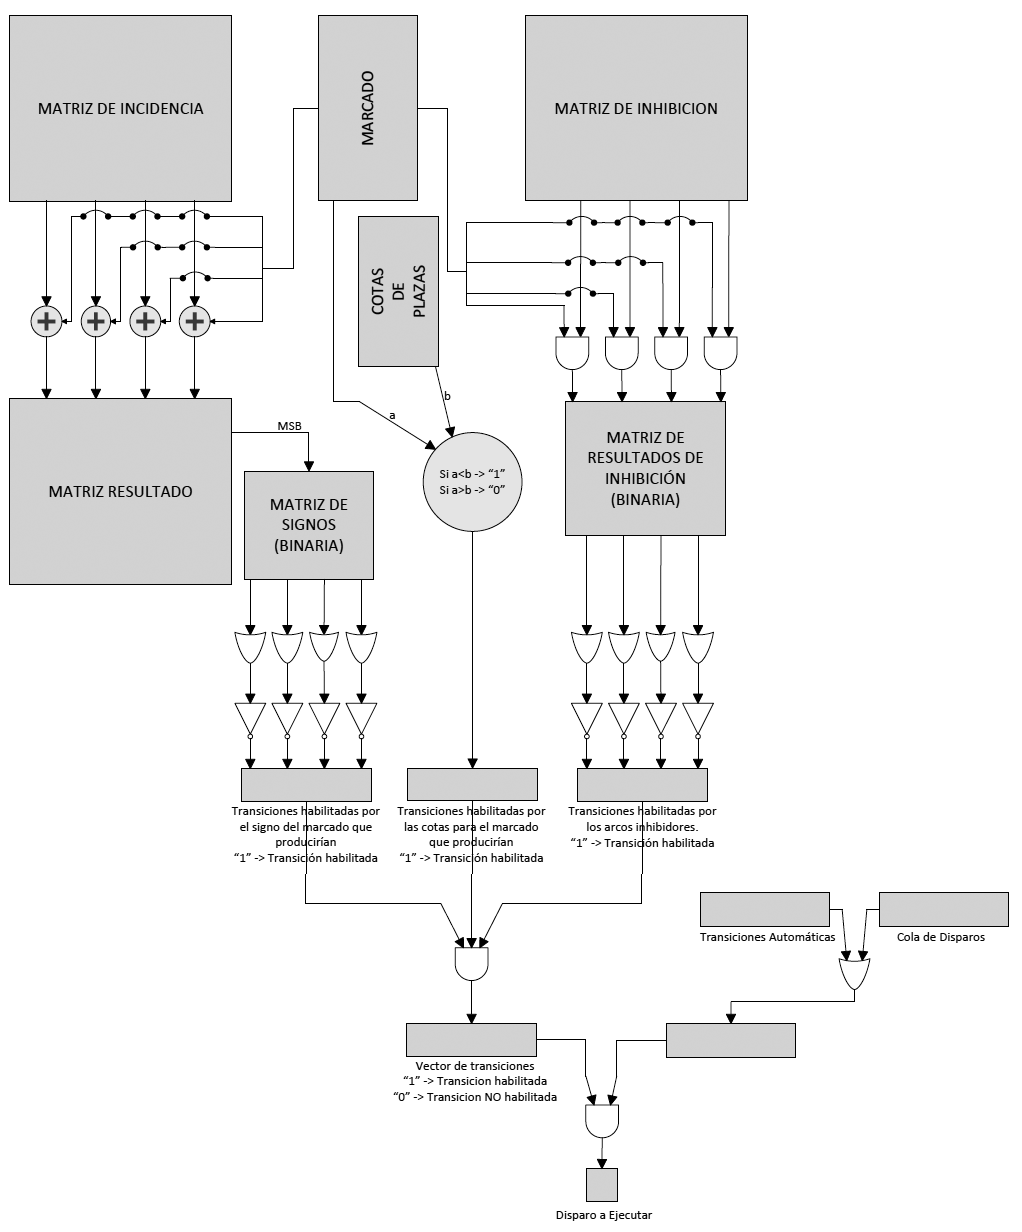
\includegraphics[width=1\linewidth,keepaspectratio]{./desarrollo/diseno_implementacion/img/diseno09}
					\caption{Implementaci�n del Procesador de Redes de Petri}
					\label{fig:diseno09}
				\end{figure}
			
			La matriz de incidencia tiene \emph{P} filas y \emph{T} columnas (\emph{P} es el numero de plazas y \emph{T} es el numero de columnas). Al disparar una transici�n \emph{$t_i$} lo que sucede es que la columna \emph{i} de la matriz se suma con el vector de marcado actual determinando el nuevo marcado. Esto se debe a que los disparos son simples, ejecutan una �nica transici�n. Por esta raz�n, un vector de disparo es un vector con todos sus elementos igual a cero exceptuando que corresponde con la transici�n que desea dispararse. Esto hace que la multiplicaci�n entre la matriz de incidencia y el vector de disparo se transforme una simple selecci�n de columna de la matriz. Esto reduce notablemente la complejidad del hardware.
				
			Dado que existen \emph{T} transiciones, en este procesador de Redes de Petri, se arma una nueva matriz llamada \textbf{\emph{Matriz Resultado}}. Cada columna \emph{k} de esta nueva matriz resulta de sumar la columna \emph{k} de la matriz de incidencia con el vector de marcado. De esta manera, cada columna de la Matriz Resultado es un posible nuevo marcado. Una vez obtenida esta matriz de resultados, se deben detectar valores negativos, cada columna de la matriz representa un posible nuevo marcado y como tal, no debe tener elementos negativos dado que esto indicar�a una cantidad negativa de tokens en una plaza. Para ello, se construye una nueva matriz binaria; cada elemento de esta matriz se corresponde con el bit m�s significativo del elemento de la matriz de resultados. Esta matriz se llama \textbf{\emph{Matriz de Signo}}.
				
			Al mismo tiempo, el vector marcado es operado con la matriz de inhibici�n para determinar si alguna transici�n deja de estar sensibilizada a causa de un arco inhibidor. Como lo determina la ecuaci�n, se realiza una operaci�n \emph{AND} entre el vector de marcado y cada columna de la matriz de inhibici�n. De aqu� surge una nueva matriz, la \textbf{\emph{Matriz de Resultados de Inhibici�n}}, que almacena los resultados de la operaci�n \emph{AND} antes descripta.

			De manera similar, comparando cada elemento del marcado con cada elemento del vector de cotas de plazas, se forma una tercera matriz, \textbf{\emph{matriz de resultados de cotas}}. Esta matriz, tendr� un \emph{1} en el elemento \emph{$a_{ij}$}, significar�a que el posible nuevo marcado que generar�a la transici�n \emph{$t_{j}$} sobre la plaza \emph{$p_{i}$} no superar�a la cota impuesta para esa plaza. 
			\clearpage
			\begin{lstlisting}	
/*****DETERMINACION DE LOS NUEVOS POSIBLES ESTADOS*****/

	//Determinacion de la matriz "resultado".	
	integer columnas;
	integer filas;
	always @(posedge Bus2IP_Clk)
	begin
		for (columnas=0 ; columnas<cant_transiciones ; columnas=columnas+1) //Recorro columnas
		begin
			for (filas=0 ; filas<cant_plazas ; filas=filas+1) // Recorro filas
			begin
				resultado[filas][columnas] = marcado[filas] + matriz_incidencia[filas][columnas]; //Ecuacion
				// Verificacion habilitacion por signo - Creaci�n de matriz
					sign_matrix [columnas][filas] = resultado[filas][columnas][tamano_de_elementos-1];
				//Verificacion habilitacion por inhibicion - Creaci�n de matriz
					inhibe_matrix [columnas][filas] = (|marcado[filas]) & matriz_inhibicion[filas][columnas];
				// Verificacion de habilitacion por cotas - Creaci�n de matriz
					if (resultado[filas][columnas][tamano_de_elementos-1]==1'b0 && resultado[filas][columnas] > cotas_plazas[filas]) // Verifico si supero la cota
					begin
						limit_matrix [columnas][filas] = 1'b0; // Cota SI superada
					end
					else  limit_matrix [columnas][filas] = 1'b1; // Cota NO superada 
			end //Fin for recorre filas
		end //Fin for recorre columnas
	end	
			\end{lstlisting}

			Con estas matrices generadas, se arman tres vectores, el vector de habilitaci�n por signo, el vector de habilitaci�n por inhibici�n y el vector de habilitaci�n por cotas. El \textbf{\emph{vector de habilitaci�n por signo}}, se forma a partir de una \emph{NOR} entre todos los elementos de cada columna de la \emph{Matriz de Signo}. Dado que cada elemento de la matriz de signo es el bit de signo del elemento correspondiente en la matriz de resultado, un valor \emph{1} indicar�a que ese elemento es negativo. Luego, la operaci�n \emph{NOR} detectar�a si en esa columna existe uno o m�s valores negativos. De esta manera, resulta un vector cuya cantidad de elementos es el numero de transiciones y un \emph{1} en el elemento \emph{i} indicar�a que la transici�n \emph{$t_i$} producir�a un marcado sin valores negativos.
			\begin{lstlisting}
for (columnas_habilitaciones=0 ; columnas_habilitaciones<cant_transiciones ; columnas_habilitaciones=columnas_habilitaciones+1) //Recorro columnas
begin
	/*SIGNO*/
	//Determinacion del vector de habilitacion de transiciones segun el "signo"
	t_enable_sign [columnas_habilitaciones] = ~(|(sign_matrix[columnas_habilitaciones][cant_plazas-1:0]));
end
			\end{lstlisting}	

			De manera similar, una operaci�n \emph{NOR} sobre cada columna de la \emph{matriz de resultados de inhibici�n} forma el \textbf{\emph{vector de habilitaci�n por inhibici�n}}. Un valor \emph{1} en el elemento \emph{$a{ij}$} de la \emph{matriz de resultados de inhibici�n} indicar�a que la plaza \emph{$p_i$} contiene elementos y esta unida con un arco inhibidor a la transici�n \emph{$t_j$}. Por lo tanto, esta ultima transici�n no esta sensibilizada. El vector de habilitaci�n por inhibici�n tendr� un \emph{1} en el elemento \emph{j} si es que la transici�n \emph{$t_j$} esta sensibilizada de acuerdo a los arcos inhibidores.
			\begin{lstlisting}
for (columnas_habilitaciones=0 ; columnas_habilitaciones<cant_transiciones ; columnas_habilitaciones=columnas_habilitaciones+1) //Recorro columnas
begin
	/*ARCOS INHIBIDORES*/
	//Determinacion del vector de habilitacion de transicones segun los "arcos inhibidores"
	t_enable_inhibicion [columnas_habilitaciones] = ~(|(inhibe_matrix[columnas_habilitaciones][cant_plazas-1:0]));
end
			\end{lstlisting}
				
			Aplicando una operaci�n \emph{OR} sobre todos los elementos de cada columna de la \emph{matriz de resultados de cotas}, se forma el \textbf{\emph{vector de habilitaci�n por cotas}} en el cual un \emph{1} en el elemento \emph{j} indica que la transici�n \emph{$t_j$} esta sensibilizada seg�n las cotas de plazas.	
			\begin{lstlisting}
for (columnas_habilitaciones=0 ; columnas_habilitaciones<cant_transiciones ; columnas_habilitaciones=columnas_habilitaciones+1) //Recorro columnas
begin
	/*COTAS*/
	//Determinacion del vector de habilitacion de transicones segun las "cotas de plazas"
	t_enable_limit [columnas_habilitaciones] = &(limit_matrix[columnas_habilitaciones][cant_plazas-1:0]);
end
			\end{lstlisting}	

			Los tres vectores de habilitaci�n de transiciones antes mencionados generan a trav�s de una operaci�n \emph{AND} el \textbf{\emph{vector de transiciones sensibilizadas}}. De esta manera, a cada cambio en el marcado de la Red de Petri se determinan cuales son las transiciones sensibilizadas. Esta informaci�n es comparada con la cola de disparos que esperan ser ejecutados y en caso de haber coincidencia, se procede a la ejecuci�n del disparo solicitado.	
			\begin{lstlisting}	
//Determinacion de las transciones habilitadas, disparos posibles
t_sensibilizadas=t_enable_sign & t_enable_inhibicion & t_enable_limit;
			\end{lstlisting}
					
			Obtenido el vector de transiciones sensibilizadas, como lo indica la Figura \ref{fig:diseno09} de la p�gina \pageref{fig:diseno09}, se verifica si el disparo de alguna de �stas transiciones est� solicitado (se encuentra en la cola de entrada de disparos) o, si la transici�n es autom�tica y no se necesita una solicitud para ejecutar su disparo.

			La ejecuci�n de un disparo consiste en actualizar el vector de marcado de la red con la columna correspondiente de la matriz de resultado. Adem�s, el disparo que se ha ejecutado se carga en la cola de disparos de salida y espera ser retirado.
		
		\subsubsection{Retiro de un disparo ejecutado}		
			
			El retiro de un disparo que ya ha sido ejecutado requiere de dos pasos, un proceso que solicito que se dispare una transici�n, debe consultar si el disparo ya se ejecuto y posteriormente, en caso afirmativo, debe remover este disparo de la cola. Para este proceso se pens� en utilizar el mismo sistema que cuando se desea cargar un nuevo disparo en la cola de entrada.
				
				\begin{figure}[ht]
					\centering
					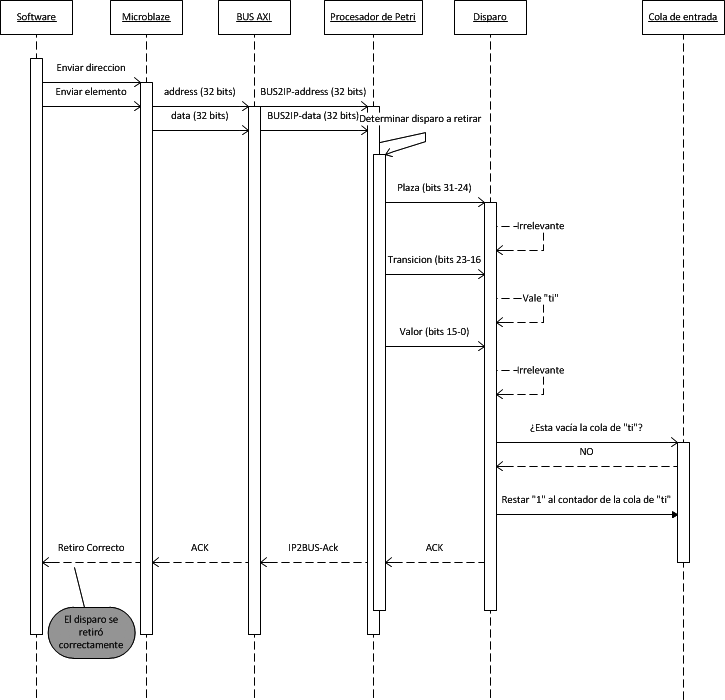
\includegraphics[width=1\linewidth,keepaspectratio]{./desarrollo/diseno_implementacion/img/diseno10}
					\caption{Diagrama de secuencia del retiro de un disparo de la cola de salida}
					\label{fig:diseno10}
				\end{figure}
				
			Se utiliza la palabra definida en la Figura \ref{fig:diseno07} al igual que en el proceso de carga de datos y de llegada de nuevos disparos. En esta palabra de 32 bits, el proceso indica sobre que transici�n desea consultar su ejecuci�n y el retiro de la cola de disparos de salida. Adem�s, esta palabra se acompa�a con una direcci�n que indica que lo que se desea realizar es el retiro de un disparo. Cuando el procesador reconoce la direcci�n y la palabra necesaria para esta operaci�n, consulta la cola del disparo solicitado. Si la cola contiene disparos que esperan salir, se decrementa un unidad (retira un disparo) y se env�a un ACK indicando al software que el disparo hab�a sido ejecutado y que adem�s, fue retirado de la cola. Si el software NO recibe el ACK entiende que su disparo no ha sido ejecutado aun debe consultar nuevamente mas tarde.
				
	\subsection{Verificaci�n}
		
		Para la verificaci�n del funcionamiento de esta primera etapa se ha dise�ado e implementado una prueba en Verilog. En esta prueba se realiza la carga de una Red de Petri simple y sencilla y luego solicita una serie de disparos verificando que la red responda de manera correcta.
			\begin{figure}[H]
				\centering
				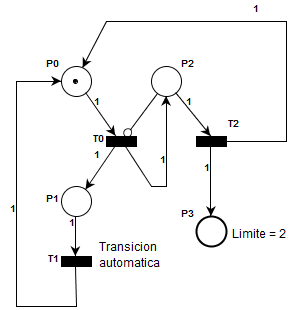
\includegraphics[width=0.5\linewidth,keepaspectratio]{./desarrollo/diseno_implementacion/img/diseno11}
				\caption{Red de Petri para la verificaci�n de la primera etapa de desarrollo}
				\label{fig:diseno11}
			\end{figure}
		
		La red de la \ref{fig:diseno11} ha sido dise�ada solo para que cumpla con ciertas propiedades necesarias para comprobar el correcto funcionamiento del procesador de Redes de Petri. Estas propiedades son:
			\begin{itemize}
			  \item Utilizar arcos inhibidores.
			  \item Tener transiciones autom�ticas.
			  \item Tener plazas con l�mites en la cantidad de tokens.
			  \item Que en alg�n momento varias transiciones est�n sensibilizadas simult�neamente.
			\end{itemize}			
				
		\subsubsection{Carga de datos}
		
			Lo primero que se debe realizar es la carga de los datos necesarios en el procesador. En el test de carga de datos, se utilizan una serie de par�metros para representar las direcciones de cada estructura.		

			\begin{lstlisting}
localparam m_incidencia=32'b00000000000000000000000000000001;
localparam m_inhibicion=32'b00000000000000000000000000000010;
localparam m_marcado=32'b00000000000000000000000000000100;
localparam p_cotas=32'b00000000000000000000000000001000;
localparam t_automatica=32'b00000000000000000000000000010000;
localparam new_disparo=32'b00000000000000000000000000100000;
localparam sacardisparo=32'b00000000000000000000000001000000;
localparam error=32'b00000000000000000000000000000111;
			\end{lstlisting}
			
			\begin{itemize}
			  	\item \emph{Carga del vector de marcado inicial:}
			  		El vector de marcado inicial, tiene la siguiente forma:
			  		\begin{equation}
			  			m_0 = \begin{bmatrix}
			  					1 \\
			  					0 \\
			  					0 \\
			  					0
			  				\end{bmatrix}
			  		\end{equation}
			  		La carga de estos valores en el procesador de Redes de Petri se realiza a trav�s del test en Verilog de la siguiente manera:
					\begin{lstlisting}			  		
//Marcado inicial [0]
	@(posedge clk)
	address 	= m_marcado;
	//Plazas: 00000000=00H - Transiciones: 00000000=00H - Elemento: 0000000000000001
	bus_in 	= 32'h00000001;
	#20;
//Marcado inicial [1]
	@(posedge clk)
	address 	= m_marcado;
	//Plazas: 00000001=01H - Transiciones: 00000000=00H - Elemento: 0000000000000000
	bus_in 	= 32'h01000000;	
	#20;
//Marcado inicial [2]
	@(posedge clk)
	address 	= m_marcado;
	//Plazas: 00000010=02H - Transiciones: 00000000=00H - Elemento: 0000000000000000
	bus_in 	= 32'h02000000;	
	#20;
//Marcado inicial [3]
	@(posedge clk)
	address 	= m_marcado;
	//Plazas: 00000011=03H - Transiciones: 00000000=00H - Elemento: 0000000000000000
	bus_in 	= 32'h03000000;	
	#20;
					\end{lstlisting}			  		
			  		
					Recordando los par�metros antes mencionados, en la Figura \ref{fig:diseno12} se encuentra una imagen de la simulaci�n en la cual se pasa el valor \emph{4H} en la entrada \emph{address} (este valor corresponde al marcado inicial). Simult�neamente, se sit�a en el bus el valor a cargar en el primer elemento de vector de marcado inicial.
			  		\begin{figure}[H]
						\centering
						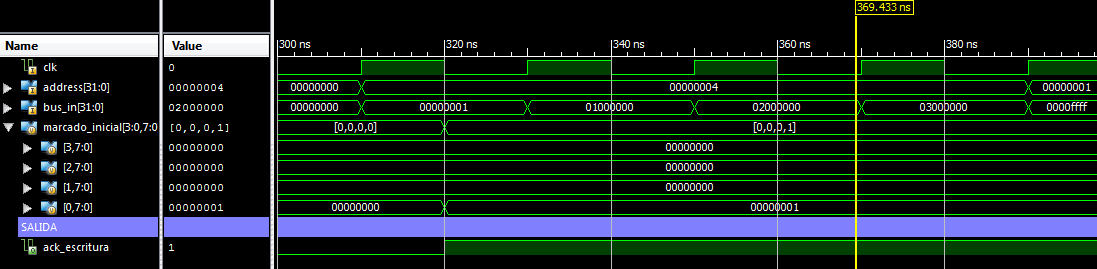
\includegraphics[width=0.9\linewidth,keepaspectratio]{./desarrollo/diseno_implementacion/img/diseno12}
						\caption{Simulaci�n de la carga del vector de marcado inicial}
						\label{fig:diseno12}
					\end{figure}
			  		En la imagen anterior, es posible observar el valor final de vector marcado inicial, notando que coincide con el valor que se deseaba cargar\footnote{La columna \emph{value} de la Figura representa el valor de la variable en el instante marcado por la l�nea amarilla.}. En el momento de la carga del primer elemento del vector de marcado inicial, se puede notar que medio ciclo despu�s de colocar el valor en el bus, se encuentra cargado en la estructura correspondiente.
			  		
			  	\item \emph{Carga de la matriz de incidencia:}
			  		La matriz de incidencia para la Red de Petri de la Figura \ref{fig:diseno11} 
			  		tiene la siguiente forma:
			  		\begin{equation}
			  			I = \begin{bmatrix}
			  					-1 & 1  & 1  \\
			  					1  & -1 & 0  \\
			  					1  & 0  & -1 \\
			  					0  & 0  & 1
			  				\end{bmatrix}
			  		\end{equation}
			  		La carga de estos valores en el procesador de Redes de Petri se realiza a trav�s del test en Verilog de la siguiente manera:
			  		\begin{lstlisting}	
//Matriz de incidencia [0][0]
	@(posedge clk)
	address 	= m_incidencia;
	//Plazas: 00000000=00H - Transiciones: 00000000=00H - Elemento: 1111111111111111
	bus_in 	= 32'h0000FFFF;	
	#20
//Matriz de incidencia [0][1]
	@(posedge clk)
	address 	= m_incidencia;
	//Plazas: 00000000=00H - Transiciones: 00000001=01H - Elemento: 0000000000000001
	bus_in 	= 32'h00010001;	
	#20;
//Matriz de incidencia [0][2]
	@(posedge clk)
	address 	= m_incidencia;
	//Plazas: 00000000=00H - Transiciones: 00000010=02H - Elemento: 0000000000000001
	bus_in 	= 32'h00020001;
	#20;	
//Matriz de incidencia [1][0]
	@(posedge clk)
	address 	= m_incidencia;
	//Plazas: 00000001=01H - Transiciones: 00000000=00H - Elemento: 0000000000000001
	bus_in 	= 32'h01000001;	
	#20;
//Matriz de incidencia [1][1]
	@(posedge clk)
	address 	= m_incidencia;
	//Plazas: 00000001=01H - Transiciones: 00000001=01H - Elemento: 1111111111111111
	bus_in 	= 32'h0101FFFF;	
	#20;
//Matriz de incidencia [1][2]
	@(posedge clk)
	address 	= m_incidencia;
	//Plazas: 00000001=01H - Transiciones: 00000010=02H - Elemento: 0000000000000000
	bus_in 	= 32'h01020000;	
	#20;
//Matriz de incidencia [2][0]
	@(posedge clk)
	address 	= m_incidencia;
	//Plazas: 00000010=02H - Transiciones: 00000000=00H - Elemento: 0000000000000001
	bus_in 	= 32'h02000001;	
	#20;
//Matriz de incidencia [2][1]
	@(posedge clk)
	address 	= m_incidencia;
	//Plazas: 00000010=02H - Transiciones: 00000001=01H - Elemento: 0000000000000000
	bus_in 	= 32'h02010000;	
	#20;
//Matriz de incidencia [2][2]
	@(posedge clk)
	address 	= m_incidencia;
	//Plazas: 00000010=02H - Transiciones: 00000010=02H - Elemento: 1111111111111111
	bus_in 	= 32'h0202FFFF;	
	#20;	
//Matriz de incidencia [3][0]
	@(posedge clk)
	address 	= m_incidencia;
	//Plazas: 00000011=03H - Transiciones: 00000000=00H - Elemento: 0000000000000000
	bus_in 	= 32'h03000000;	
	#20;
//Matriz de incidencia [3][1]
	@(posedge clk)
	address 	= m_incidencia;
	//Plazas: 00000011=03H - Transiciones: 00000001=01H - Elemento: 0000000000000000
	bus_in 	= 32'h03010000;	
	#20;
//Matriz de incidencia [3][2]
	@(posedge clk)
	address 	= m_incidencia;
	//Plazas: 00000011=03H - Transiciones: 00000010=02H - Elemento: 0000000000000001
	bus_in 	= 32'h03020001;	
	#20;
					\end{lstlisting}
			  		
					La siguiente imagen, mostrara que la matriz de incidencia a sido efectivamente cargada.	
					\begin{figure}[H]
						\centering
						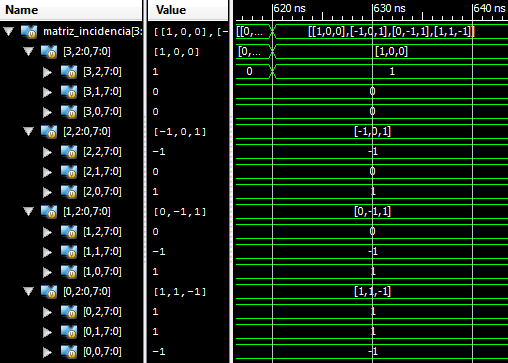
\includegraphics[width=0.6\linewidth,keepaspectratio]{./desarrollo/diseno_implementacion/img/diseno13}
						\caption{Valor que alcanza la matriz de incidencia luego del proceso de carga}
						\label{fig:diseno13}
					\end{figure}
					
				\item \emph{Carga de la matriz de inhibici�n}
					La matriz de arcos inhibidores resulta:		  		
			  		\begin{equation}
			  			H = \begin{bmatrix}
			  					0 & 0 & 0 \\
			  					0 & 0 & 0 \\
			  					1 & 0 & 0 \\
			  					0 & 0 & 0
			  				\end{bmatrix}
			  		\end{equation}
			  		La carga de estos valores en el procesador de Redes de Petri se realiza a trav�s del test en Verilog de la siguiente manera:
			  		\begin{lstlisting}	
//Matriz de inhibicion [0][0]
	@(posedge clk)
	address 	= m_inhibicion;
	//Plazas: 00000000=00H - Transiciones: 00000000=00H - Elemento: 0000000000000000
	bus_in 	= 32'h00000000;	
	#20;
//Matriz de inhibicion [0][1]
	@(posedge clk)
	address 	= m_inhibicion;
	//Plazas: 00000000=00H - Transiciones: 00000001=01H - Elemento: 0000000000000000
	bus_in 	= 32'h00010000;	
	#20;
//Matriz de inhibicion [0][2]
	@(posedge clk)
	address 	= m_inhibicion;
	//Plazas: 00000000=00H - Transiciones: 00000010=02H - Elemento: 0000000000000000
	bus_in 	= 32'h00020000;	
	#20;	
//Matriz de inhibicion [1][0]
	@(posedge clk)
	address 	= m_inhibicion;
	//Plazas: 00000001=01H - Transiciones: 00000000=00H - Elemento: 0000000000000000
	bus_in 	= 32'h01000000;	
	#20;
//Matriz de inhibicion [1][1]
	@(posedge clk)
	address 	= m_inhibicion;
	//Plazas: 00000001=01H - Transiciones: 00000001=01H - Elemento: 0000000000000000
	bus_in 	= 32'h01010000;	
	#20;
//Matriz de inhibicion [1][2]
	@(posedge clk)
	address 	= m_inhibicion;
	//Plazas: 00000001=01H - Transiciones: 00000010=02H - Elemento: 0000000000000000
	bus_in 	= 32'h01020000;	
	#20;	
//Matriz de inhibicion [2][0]
	@(posedge clk)
	address 	= m_inhibicion;
	//Plazas: 00000010=02H - Transiciones: 00000000=00H - Elemento: 0000000000000001
	bus_in 	= 32'h02000001;	
	#20;
//Matriz de inhibicion [2][1]
	@(posedge clk)
	address 	= m_inhibicion;
	//Plazas: 00000010=02H - Transiciones: 00000001=01H - Elemento: 0000000000000000
	bus_in 	= 32'h02010000;	
	#20;
//Matriz de inhibicion [2][2]
	@(posedge clk)
	address 	= m_inhibicion;
	//Plazas: 00000010=02H - Transiciones: 00000010=02H - Elemento: 0000000000000000
	bus_in 	= 32'h02020000;	
	#20;	
//Matriz de inhibicion [3][0]
	@(posedge clk)
	address 	= m_inhibicion;
	//Plazas: 00000011=03H - Transiciones: 00000000=00H - Elemento: 0000000000000000
	bus_in 	= 32'h03000001;	
	#20;
//Matriz de inhibicion [3][1]
	@(posedge clk)
	address 	= m_inhibicion;
	//Plazas: 00000011=03H - Transiciones: 00000001=01H - Elemento: 0000000000000000
	bus_in 	= 32'h03010000;	
	#20;
//Matriz de inhibicion [3][2]
	@(posedge clk)
	address 	= m_inhibicion;
	//Plazas: 00000011=03H - Transiciones: 00000010=02H - Elemento: 0000000000000000
	bus_in 	= 32'h03020000;	
	#20;
					\end{lstlisting}
					De manera similar al caso anterior, se ver� como resulta la matriz de inhibici�n:
					\begin{figure}[H]
						\centering
						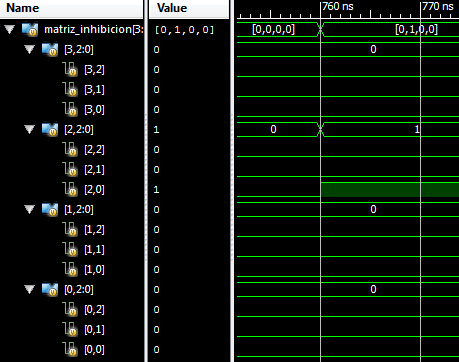
\includegraphics[width=0.7\linewidth,keepaspectratio]{./desarrollo/diseno_implementacion/img/diseno14}
						\caption{Valor que alcanza la matriz de inhibici�n luego del proceso de carga}
						\label{fig:diseno14}
					\end{figure}
				
				\item \emph{Carga del vector de cotas en plazas}	
					El vector de cotas de plazas es:
					\begin{equation}
			  			\begin{bmatrix}
			  				P_0 \\
			  				P_2 \\
			  				P_2 \\
			  				P_3 
			  			\end{bmatrix} 
			  			=
			  			\begin{bmatrix}
			  				max \\
			  				max \\
			  				max \\
			  				2 	
			  			\end{bmatrix} 
			  		\end{equation}
					La carga de estos valores en el procesador de Redes de Petri se realiza a trav�s del test en Verilog de la siguiente manera:
					\begin{lstlisting}
//Vector de cotas [0]
	@(posedge clk)
	address 	= p_cotas;
	//Plazas: 00000000=00H - Transiciones: 00000000=00H - Elemento: 1111111111111111
	bus_in	= 32'h0000FFFF;	
	#20;
//Vector de cotas [1]
	@(posedge clk)
	address 	= p_cotas;
	//Plazas: 00000001=01H - Transiciones: 00000000=00H - Elemento: 1111111111111111
	bus_in	= 32'h0100FFFF;	
	#20;
//Vector de cotas [2]
	@(posedge clk)
	address 	= p_cotas;
	//Plazas: 00000010=02H - Transiciones: 00000000=00H - Elemento: 1111111111111111
	bus_in	= 32'h0200FFFF;	
	#20;
//Vector de cotas [3]
	@(posedge clk)
	address 	= p_cotas;
	//Plazas: 00000011=03H - Transiciones: 00000000=00H - Elemento: 0000000000000010
	bus_in	= 32'h03000002;	
	#20;
					\end{lstlisting}
					
					En la simulaci�n observamos lo siguiente:
					\begin{figure}[H]
						\centering
						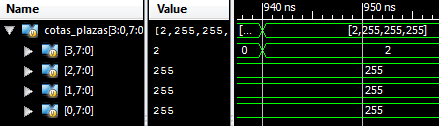
\includegraphics[width=0.55\linewidth,keepaspectratio]{./desarrollo/diseno_implementacion/img/diseno15}
						\caption{Valor que alcanza el vector de cotas de plazas luego del proceso de carga}
						\label{fig:diseno15}
					\end{figure}
				
				\item \emph{Carga del vector de transiciones autom�ticas}	
					El vector de transiciones autom�ticas tiene la siguiente forma:
					\begin{equation}
			  			\begin{bmatrix}
			  				T_0 \\
			  				T_2 \\
			  				T_2
			  			\end{bmatrix} 
			  			=
			  			\begin{bmatrix}
			  				0 \\
			  				1 \\
			  				0
			  			\end{bmatrix} 
			  		\end{equation}
			  		La carga de estos valores en el procesador de Redes de Petri se realiza a trav�s del test en Verilog de la siguiente manera:
			  		\begin{lstlisting}
//Transicion Automatica [0]
	@(posedge clk)
	address 	= t_automatica;
	//Plazas: 00000000=00H - Transiciones: 00000000=00H - Elemento: 0000000000000000
	bus_in	= 32'h00000000;	
	#20;
//Transicion Automatica[1]
	@(posedge clk)
	address 	= t_automatica;
	//Plazas: 00000000=01H - Transiciones: 00000001=01H - Elemento: 0000000000000001
	bus_in	= 32'h00010001;	
	#20;
//Transicion Automatica[2]
	@(posedge clk)
	address 	= t_automatica;
	//Plazas: 00000000=01H - Transiciones: 00000010=02H - Elemento: 0000000000000000
	bus_in	= 32'h00020000;	
	#20;
					\end{lstlisting}
					Observando como resulta este vector en la simulaci�n:
					\begin{figure}[H]
						\centering
						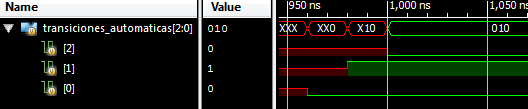
\includegraphics[width=0.55\linewidth,keepaspectratio]{./desarrollo/diseno_implementacion/img/diseno16}
						\caption{Valor que alcanza el vector de transiciones autom�ticas luego del proceso de carga}
						\label{fig:diseno16}
					\end{figure}			  		
			\end{itemize}
	
		\subsubsection{Secuencia de disparos}
			
			A continuaci�n, se presentar� la secuencia de disparos que se aplicar� sobre la Red de Petri de la \ref{fig:diseno11}. Cada disparo que se aplique, producir� un marcado que se comparara con el obtenido en un simulador de Redes de Petri (PIPE versi�n 4).
			\begin{center}
				$S = { T2, T0, T0, T0, T2, T0 }$
			\end{center}
			Se debe notar que la transici�n \emph{T1} no se encuentra incluida en la lista debido a que fue marcada como autom�tica, por lo tanto, no es necesario hacer un pedido para que sea disparada. La secuencia de disparos ha sido elegida con el fin de que se compruebe el comportamiento del procesador de Redes de Petri en diversas circunstancias. La Figura \ref{fig:diseno16} muestra la simulaci�n del �ltimo dato cargado en el Procesador de Redes de Petri. Como se observa en dicha Figura, en el instante de los 1000 ns el procesador ya esta listo para comenzar recibir solicitudes de disparos. La afirmaci�n anterior es demostrada por la siguiente Figura (\ref{fig:diseno17}).
				\begin{figure}[H]
					\centering
					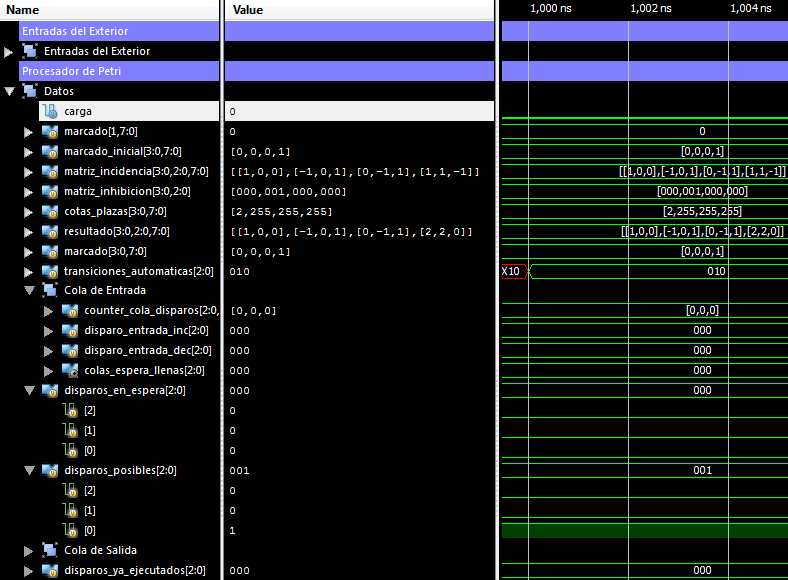
\includegraphics[width=0.75\linewidth,keepaspectratio]{./desarrollo/diseno_implementacion/img/diseno17}
					\caption{Estado del Procesador de Redes de Petri luego de la carga de todos los datos}
					\label{fig:diseno17}
				\end{figure}
			Se observa que al comenzar, el procesador de Petri determina que el �nico disparo posible es el de la transici�n \emph{0}, coincidiendo con el simulador.
				\begin{figure}[H]
					\centering
					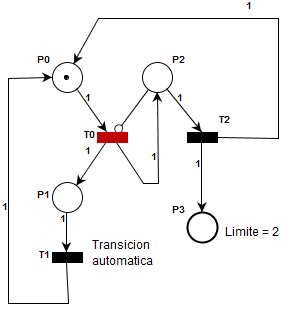
\includegraphics[width=0.3\linewidth,keepaspectratio]{./desarrollo/diseno_implementacion/img/diseno18}
					\caption{Estado inicial de la Red de Petri}
					\label{fig:diseno18}
				\end{figure}
			Partiendo desde esta situaci�n, se puede comenzar a enviar la secuencia de disparos.
			
			\begin{enumerate}
				\item \emph{Solicitar el disparo de \textbf{T2}}
					
					Esta solicitud se env�a para comprobar que el procesador ubica correctamente en la cola de espera a las solicitudes de disparo para transiciones que no est�n sensibilizadas como es el caso de \emph{T2}.
					\begin{lstlisting}
//Solicito disparo de T2 -> Deber�a ir a la cola porque T2 NO esta sensibilizada
@(posedge clk)
address	= new_disparo;
//Plazas: 00000000=00H - Transiciones: 00000010=02H - Elemento: 0000000000000000
bus_in = 32'h00020000;	
@(negedge clk)
address	= error;
					\end{lstlisting}					
					\begin{figure}[H]
						\centering
						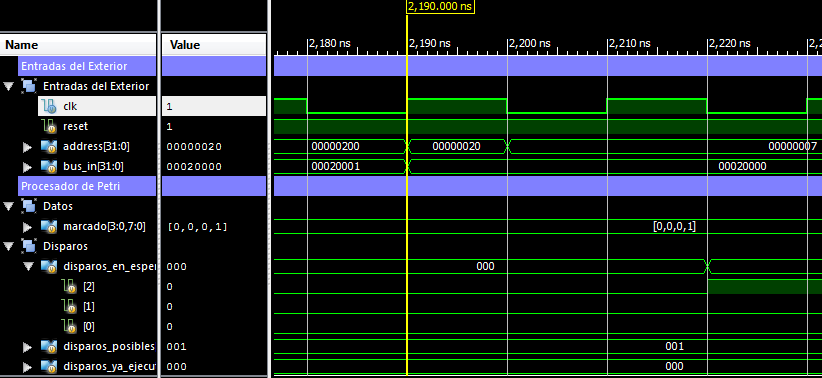
\includegraphics[width=1\linewidth,keepaspectratio]{./desarrollo/diseno_implementacion/img/diseno19}
						\caption{Simulaci�n primer disparo de la secuencia de prueba}
						\label{fig:diseno19}
					\end{figure}
				
					En la Figura \ref{fig:diseno19} la simulaci�n del procesador de Redes de Petri cuando llega la primera solicitud de disparo. Como se dijo, esta solicitud es para una transici�n que no esta sensibilizada por lo tanto, no se encuentra entre los disparos posibles y queda almacenado en la cola.
									
				\item \emph{Solicitar el disparo de \textbf{T0}}
					
					Luego, se solicita el disparo de la transici�n \emph{T0} esperando que sea disparada porque es la �nica transici�n sensibilizada.
					\begin{figure}[H]
						\centering
						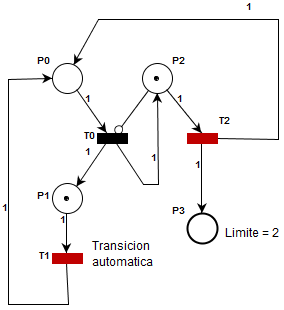
\includegraphics[width=0.4\linewidth,keepaspectratio]{./desarrollo/diseno_implementacion/img/diseno20}
						\caption{Estado esperado de la Red luego de disparar \emph{T0}}
						\label{fig:diseno20}
					\end{figure}
					Al solicitar el disparo, se observa que es cargado en la cola. Luego, como el procesador reconoce que es una solicitud sobre una transici�n que esta sensibilizada la ejecuta.					
					\begin{figure}[H]
						\centering
						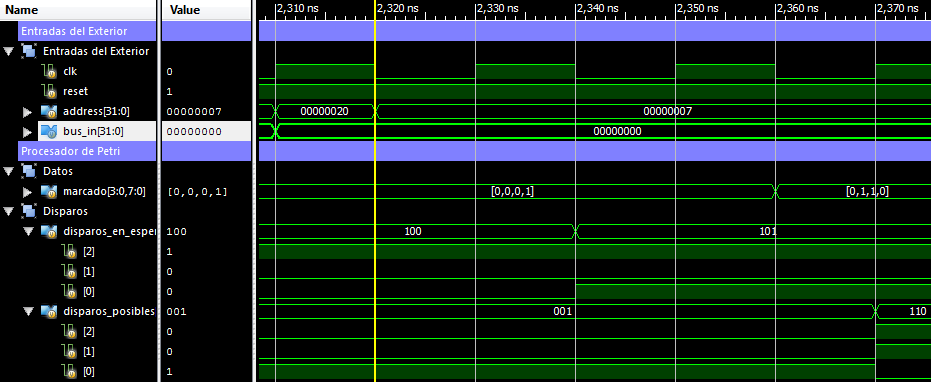
\includegraphics[width=1\linewidth,keepaspectratio]{./desarrollo/diseno_implementacion/img/diseno21}
						\caption{Solicitud y disparo de la transici�n \emph{T0}}
						\label{fig:diseno21}
					\end{figure}
					La l�nea amarilla marca el instante en el cual se pone en el bus el address correspondiente a un nuevo disparo y el valor que indica que disparo se desea solicitar. Ese nuevo dato, se coloca en el bus en un flanco positivo de reloj, el procesador de Redes de Petri recibe el dato en el flanco negativo. Luego de la recepci�n del disparo se demora un ciclo en colocar el disparo en la cola de entrada correspondiente y un ciclo en actualizar el marcado a partir de un disparo que se encuentre en la cola. 
					
					\textbf{\emph{De esta manera, se observa que cuando llega un nuevo disparo, en dos ciclos el procesador de Redes de Petri genera el cambio de estado.}} Se debe notar que luego de que el marcado cambi�, el procesador necesita medio ciclo para calcular el nuevo vector de disparos posibles.

					Luego de que la transici�n \emph{T0} se dispara, quedan sensibilizadas las transiciones \emph{T1} y \emph{T2}. Como la primera de ellas es una transici�n autom�tica y la segunda fue solicitada anteriormente, ambas se ejecutan y se actualiza el marcado.

					La Figura \ref{fig:diseno22} muestra como, luego de que el marcado fue actualizado por la transici�n \emph{T0}, la transici�n \emph{T2} que se encontraba en la cola de disparos en espera es disparada y luego la transici�n \emph{T1} que fue marcada como autom�tica. Cada uno de estos disparos, como ya estaban las solicitudes dentro del procesador, toma solo un ciclo de ejecuci�n cada uno.

					En la imagen, puede observarse como dejan de ser posibles los disparos \emph{T2} y \emph{T1} y comienza a estar sensibilizada la transici�n \emph{T0}, tambi�n se observa como se marcan estos disparos en la cola de los que ya han sido ejecutados.
					\begin{figure}[H]
						\centering
						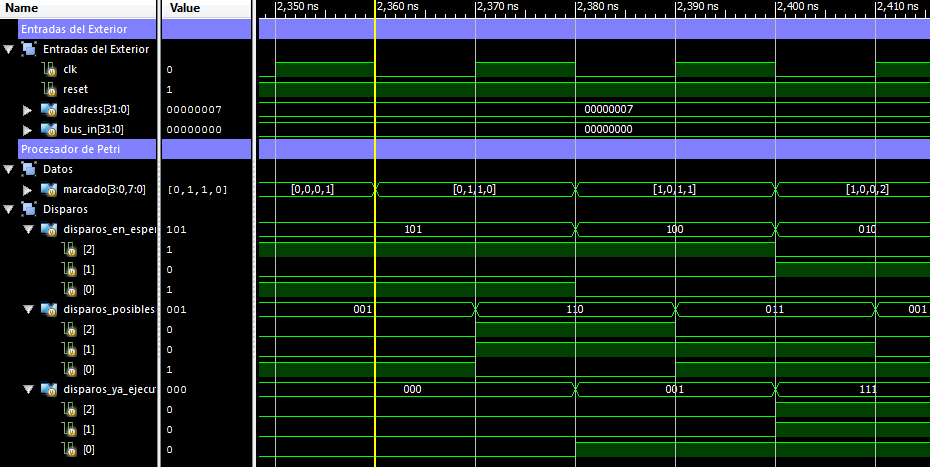
\includegraphics[width=0.75\linewidth,keepaspectratio]{./desarrollo/diseno_implementacion/img/diseno22}
						\caption{Disparo de las transiciones \emph{T0} y \emph{T2}}
						\label{fig:diseno22}
					\end{figure}
					
					\begin{figure}[H]
						\centering
						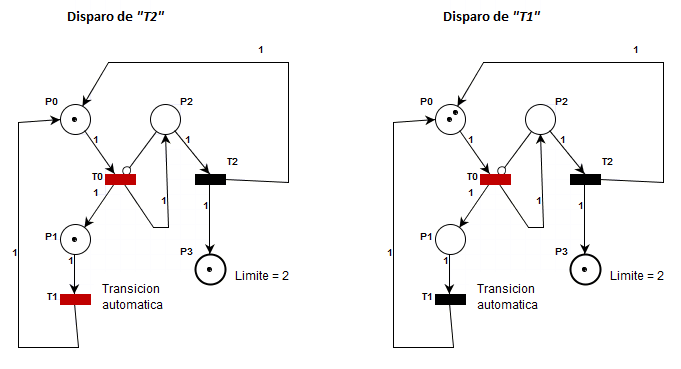
\includegraphics[width=0.75\linewidth,keepaspectratio]{./desarrollo/diseno_implementacion/img/diseno23}
						\caption{Cambios de estado en la Red de Petri}
						\label{fig:diseno23}
					\end{figure}
									
					Comparando la Figura \ref{fig:diseno22} con la Figura \ref{fig:diseno23} se observa coinciden los sucesivos marcados y las transiciones que se encuentran sensibilizadas en cada uno de ellos.
				
				\item \emph{Solicitar el disparo de \textbf{T0}}
					
					\begin{figure}[H]
						\centering
						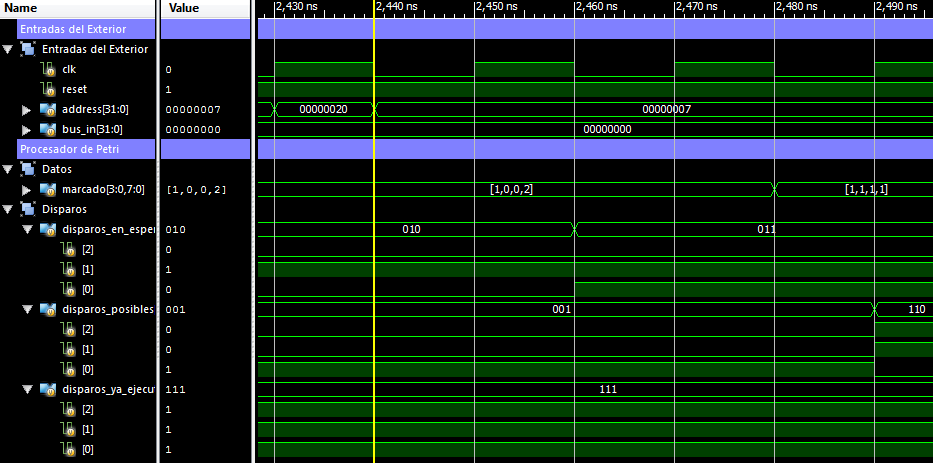
\includegraphics[width=1\linewidth,keepaspectratio]{./desarrollo/diseno_implementacion/img/diseno24}
						\caption{Segundo disparo de la transici�n \emph{T0} (simulaci�n)}
						\label{fig:diseno24}
					\end{figure}
					
					\begin{figure}[H]
						\centering
						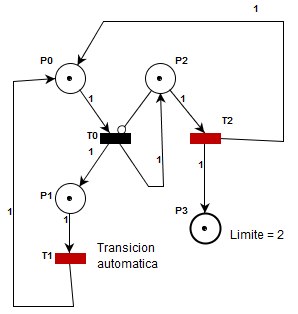
\includegraphics[width=0.5\linewidth,keepaspectratio]{./desarrollo/diseno_implementacion/img/diseno25}
						\caption{Segundo disparo de la transici�n \emph{T0} (Red de Petri)}
						\label{fig:diseno25}
					\end{figure}
					
					Se solicita el disparo de la transici�n \emph{T0} dado que esta sensibilizada. Luego, la transici�n \emph{T1} se disparar� por ser una transici�n autom�tica.
					
					\begin{figure}[H]
						\centering
						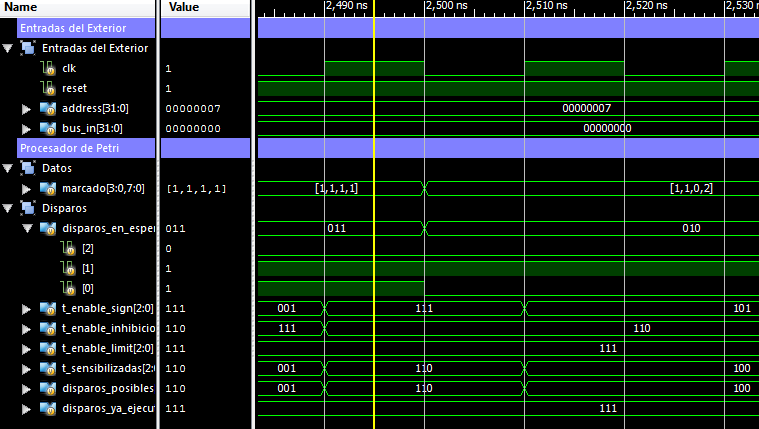
\includegraphics[width=1\linewidth,keepaspectratio]{./desarrollo/diseno_implementacion/img/diseno26}
						\caption{Disparo autom�tico de \emph{T1} (simulaci�n)}
						\label{fig:diseno26}
					\end{figure}
					
					\begin{figure}[H]
						\centering
						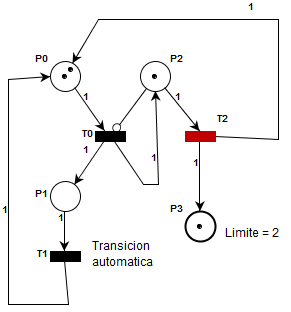
\includegraphics[width=0.4\linewidth,keepaspectratio]{./desarrollo/diseno_implementacion/img/diseno27}
						\caption{Disparo autom�tico de \emph{T1} (Red de Petri)}
						\label{fig:diseno27}
					\end{figure}
				
					En las Figuras \ref{fig:diseno26} y \ref{fig:diseno27} se observa que tras el disparo autom�tico de \emph{T1}, \emph{T0} no resulta sensibilizada por el arco inhibidor que la une a \emph{P2}.
					
				\item \emph{Solicitar el disparo de \textbf{T0}}
					
					Dado que \emph{T0} no esta sensibilizada por al solicitar su disparo, se almacenara en la cola de espera.
					
					\begin{figure}[H]
						\centering
						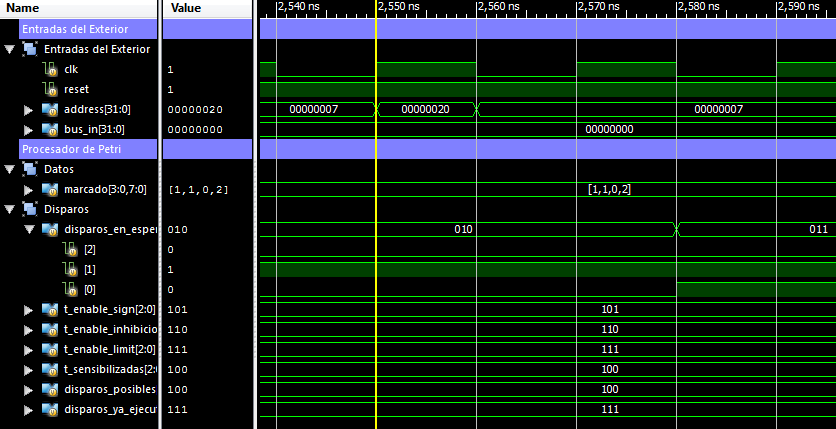
\includegraphics[width=1\linewidth,keepaspectratio]{./desarrollo/diseno_implementacion/img/diseno28}
						\caption{Solicitud de disparo de \emph{T0}}
						\label{fig:diseno28}
					\end{figure}
					
					En la Figura \ref{fig:diseno28} se observa como al solicitar el disparo de \emph{T0} queda en la cola de disparos en espera.
									
				\item \emph{Solicitar el disparo de \textbf{T2}}			  
			  
			  		La �nica transici�n sensibilizada en este momento es la transici�n \emph{T2} entonces, al solicitar su disparo se ejecutar�.
			  		
			  		\begin{figure}[H]
						\centering
						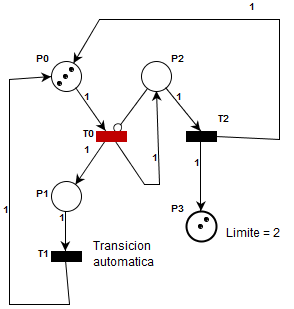
\includegraphics[width=0.4\linewidth,keepaspectratio]{./desarrollo/diseno_implementacion/img/diseno29}
						\caption{Disparo de \emph{T2} (Red de Petri)}
						\label{fig:diseno29}
					\end{figure}
			  		
			  		Al disparar la transici�n \emph{T2} la plaza \emph{P3} alcanza una cantidad de dos tokens, dado que estaba limitada a esta cantidad, la transici�n \emph{T2} ya no podr� estar sensibilizada.
			  		
			  		\begin{figure}[H]
						\centering
						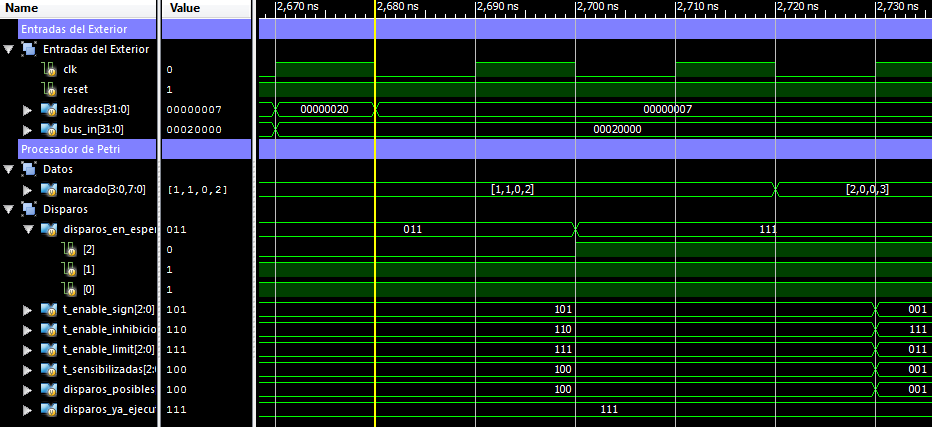
\includegraphics[width=1\linewidth,keepaspectratio]{./desarrollo/diseno_implementacion/img/diseno30}
						\caption{Disparo de \emph{T2} (simulaci�n)}
						\label{fig:diseno30}
					\end{figure}
			  		
			  		En la Figura \ref{fig:diseno30}, se observa que el vector \emph{t enable limit} indica que la transici�n \emph{T2} deja de estar sensibilizada por las cotas en las plazas.

					Como el disparo de la transici�n \emph{T0} estaba solicitado y dispararla implica que \emph{T1} quede sensibilizada y por ser autom�tica tambi�n se disparar�.
			  		
			  		\begin{figure}[H]
						\centering
						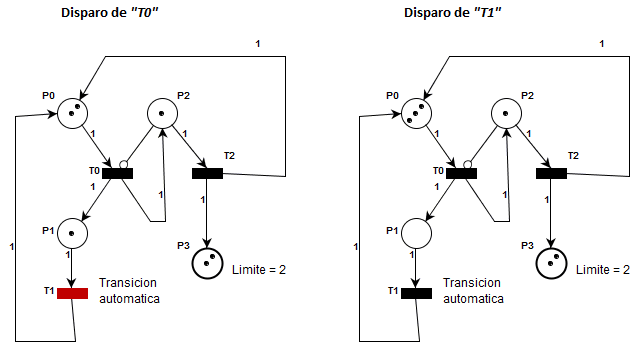
\includegraphics[width=0.8\linewidth,keepaspectratio]{./desarrollo/diseno_implementacion/img/diseno31}
						\caption{Disparos de \emph{T0} y \emph{T1} (Red de Petri)}
						\label{fig:diseno31}
					\end{figure}
			  		
			  		Tras el disparo de estas transiciones, se observa que \emph{T0} no puede estar sensibilizada debido al arco inhibidor que la une a \emph{P2}. \emph{T1} no puede sensibilizarse porque \emph{P1} no tiene tokens. Y, \emph{T2} no puede sensibilizarse porque \emph{P3} alcanz� su l�mite de tokens. La Red de Petri queda bloqueada.

					\begin{figure}[H]
						\centering
						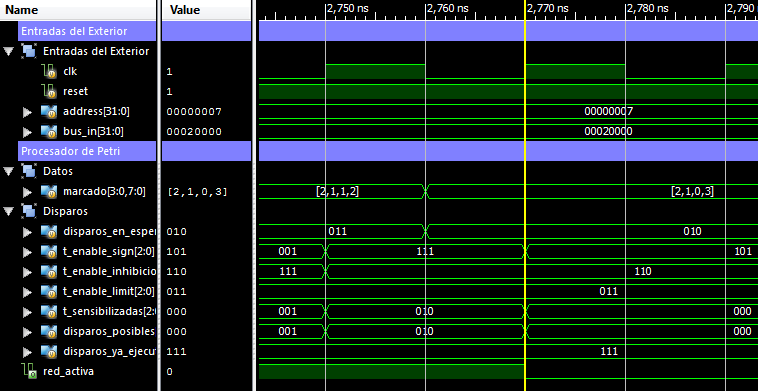
\includegraphics[width=1\linewidth,keepaspectratio]{./desarrollo/diseno_implementacion/img/diseno32}
						\caption{Disparos de \emph{T0} y \emph{T1} (simulaci�n)}
						\label{fig:diseno32}
					\end{figure}
			  		
			 		Se observa que el bit \textbf{\emph{red activa}} indica que la Red de Petri alcanz� un estado a partir del cual no puede continuar.
			  
			\end{enumerate}
			
		
	% Procesador de Petri (segunda etapa)
		%%%%%%%%%%%%%%%%%%%%%%%%%%%%%%%%%%%%%%%%%%%%%%%%%%%%%%%%%%%%%%%%%%%%%%%%%%%%%%%%%%%%%
%																					%
%	TRABAJO: Proyecto Integrador													%
%																					%
%		Titulo: 	Desarrollo de IP cores con procesamiento de Redes de Petri 		%
%					Temporales para sistemas multicore en FPGA						%
%																					%
%		Autores:	Juli�n Nonino													%
%					Carlos Renzo Pisetta											%
%		Director:	Orlando Micolini												%
%																					%
%	Parte: Desarrollo																%
%	Capitulo: Dise�o e Implementaci�n												%
%	Seccion: Procesador de Petri (segunda etapa)									%	
%	Archivo: proc_petri_segunda_etapa.tex											%
%																					%
%%%%%%%%%%%%%%%%%%%%%%%%%%%%%%%%%%%%%%%%%%%%%%%%%%%%%%%%%%%%%%%%%%%%%%%%%%%%%%%%%%%%%

% Path Imagenes: ./desarrollo/diseno_implementacion/img
% Nombre predeterminado imagenes: disenoxx
%	xx es el numero de imagen

\section{Procesador de Petri (segunda etapa)}
	\label{sec:proc_petri_segunda_etapa}

	En esta segunda etapa de implementaci�n del procesador de Redes de Petri, se agreg� 
	la capacidad de procesamiento de Redes de Petri con Tiempo.
	
	\subsection{Requerimientos}
		
		El requerimiento para esta etapa es proveer las estructuras de datos y los 
		mecanismos necesarios para ejecutar \textbf{\emph{Redes de Petri con Tiempo}}.
				
	\subsection{Arquitectura}
		
		La arquitectura del procesador de Redes de Petri en esta etapa es la misma que 
		la que se plante� al comienzo para la primera etapa. Solo se agregan elementos, 
		las estructuras de datos necesarias, el vector de \textbf{\emph{Earliest Firing Time (EFT)}}, 
		el vector de tiempo y el vector de \textbf{\emph{Latest Firing Time (LFT)}}.
		
		\newpage	
			
			\begin{figure}[H]
				\centering
				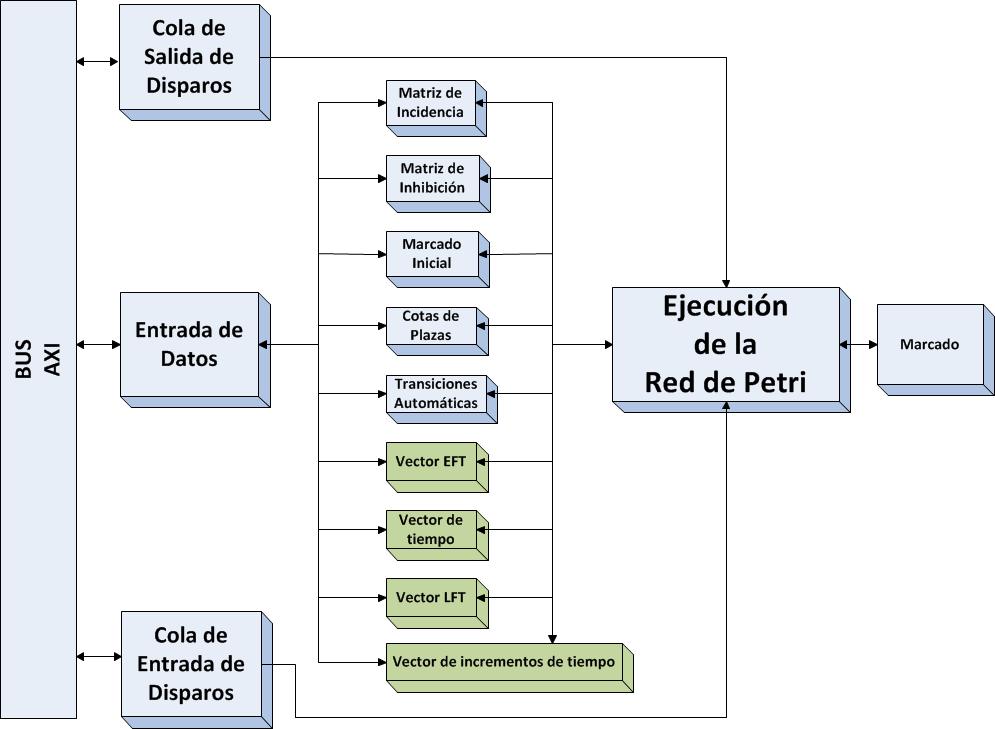
\includegraphics[width=1\linewidth,keepaspectratio]{./desarrollo/diseno_implementacion/img/diseno33}
				\caption{Arquitectura del Procesador de Redes de Petri con Tiempo}
				\label{fig:diseno33}
			\end{figure}
	
	\subsection{Estructuras de datos para Redes de Petri con Tiempo}
	
		Como se muestra en la Figura \ref{fig:diseno33} las estructuras de datos necesarias 
		para la resoluci�n de \textbf{\emph{Redes de Petri con Tiempo}} son cuatro:
		\begin{itemize}
		  	\item Vector \textbf{\emph{Earlier Firing Time (EFT)}}.
		  	\item Vector de \textbf{\emph{marcas temporales}}.
		  	\item Vector \textbf{\emph{Latest Firing Time (LFT)}}.
		  	\item Vector de \textbf{\emph{escala de incrementos de tiempo}}.
		\end{itemize}
		Los cuatro vectores tienen como cantidad de elementos el n�mero de transiciones. Los 
		tres primeros son tiene un tama�o de elementos parametrizable pero por defecto tienen 
		48 bits. El vector de escala de incrementos de tiempo, por defecto toma el un tama�o 
		de elementos de 5 bits.
			
	\subsection{Determinaci�n de disparos posibles en Redes de Petri con Tiempo}
	
		Para que un disparo sea posible en una Red de Petri, debe cumplir las condiciones dadas 
		por que todas las transiciones de las cuales toma tokens tengan la cantidad necesaria de 
		tokens, que las plazas a las cuales esta conectada con arcos inhibidores no tengan tokens 
		y que las plazas en las cuales depositan tokens no superen los limites impuestos por las 
		cotas en las plazas.
		En una \textbf{\emph{Red de Petri con Tiempo}}, adem�s de las condiciones anteriores, se 
		debe cumplir que la marca de tiempo asociada a la transici�n sea mayor o igual al l�mite 
		de tiempo inferior (\emph{EFT}) y menor o igual al l�mite de tiempo superior \emph{LFT}.
		Se debe recordar la sem�ntica temporal utilizada, el vector de tiempo asociado a una 
		transici�n, lleva cuenta del tiempo desde el instante en el que la transici�n se sensibiliz�.

		Durante el proceso de carga y en el instante en el cual este termina, las marcas de tiempo 
		de todas las transiciones valen cero. 
		Luego, a cada ciclo de reloj, si la transici�n esta sensibilizada la marca de tiempo se 
		incrementa la cantidad de unidades que indica el \emph{vector de incrementos de marcas de tiempo}.
		La marca de tiempo vuelve a cero en dos situaciones, si la transici�n es disparada o si deja 
		de estar sensibilizada.

		Una \textbf{\emph{transici�n sensibilizada}}, si no deja de estarlo, incrementar� su \emph{marca de tiempo} 
		hasta que alcance el valor indicado en el \emph{vector EFT}. A partir de dicho instante, la 
		transici�n se convierte en un \textbf{\emph{disparo posible}}. El incremento en la marca de 
		tiempo continua hasta que se solicita el disparo de la transici�n o deja de estar sensibilizada. 
		Si la marca de tiempo supera el valor indicado en el \emph{vector LFT}, y no ha sido disparada, 
		dejar� de ser un disparo posible y ya no podr� dispararse.
		
	\subsection{Verificaci�n}
		
		Para la verificaci�n del funcionamiento del procesador de Redes de Petri en esta segunda etapa, 
		considerando Redes de Petri con Tiempo, se utilizar� la siguiente Red de Petri:
		
			\begin{figure}[H]
				\centering
				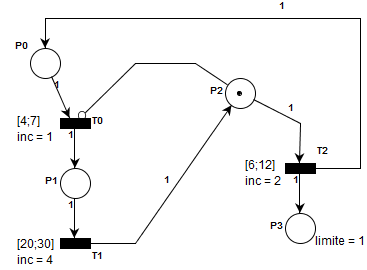
\includegraphics[width=0.5\linewidth,keepaspectratio]{./desarrollo/diseno_implementacion/img/diseno34}
				\caption{Red de Petri para la verificaci�n de la segunda etapa de desarrollo}
				\label{fig:diseno34}
			\end{figure}
		
		\subsubsection{Carga de datos}
			
			Datos de la Red de Petri de la Figura \ref{fig:diseno34}:
			\begin{center}
				\begin{tabular}{c c c}
					% Primera Fila
						% Columna Uno
							$m_0 = \begin{bmatrix}
 						  				0 \\
 						  				0 \\
   						  				1 \\
   						  				0
   									\end{bmatrix}$ 
   						& 
   						% Columna dos
   							$I = \begin{bmatrix}
 						  				-1 	& 0		& 0		\\
 						  				1 	& -1	& 0		\\
   						  				0 	& 1 	& -1	\\
   						  				0 	& 0 	& 1
   						  		\end{bmatrix}$  
   						&
   						%Columna Tres
   							$H = \begin{bmatrix}
 						  				0 & 0 & 0 \\
 						  				0 & 0 & 0 \\
   						  				1 & 0 & 0 \\
   						  				0 & 0 & 0
   						  		\end{bmatrix}$  
					\\
					%Segunda Fila
						\emph{Marcado Inicial} & \emph{Matriz de Incidencia} & \emph{Matriz de Inhibici�n} 				
					\end{tabular}
			\end{center}
			
			\begin{center}
				\begin{tabular}{c c}
					% Primera Fila
						% Columna Uno
							$\begin{bmatrix}
 						  				P_0 \\
 						  				P_1 \\
   						  				P_2 \\
   						  				P_3
   							\end{bmatrix} 
   							= 
   							\begin{bmatrix}
 						  		max \\
 						  		max \\
   						  		max \\
   						  		1
   							\end{bmatrix}$ 
   						& 
   						% Columna dos
							$\begin{bmatrix}
 						  				T_0 \\
 						  				T_1 \\
   						  				T_2 
   							\end{bmatrix} 
   							= 
   							\begin{bmatrix}
 						  		0 \\
 						  		0 \\
   						  		0
   							\end{bmatrix}$ 
					\\
					%Segunda Fila
						\emph{Vector de Cotas de Plazas} & \emph{Vector de Transiciones Autom�ticas} 				
					\end{tabular}
			\end{center}
			
			\begin{center}
				\begin{tabular}{c c c}
					% Primera Fila
						% Columna Uno
							$\begin{bmatrix}
 						  				T_0 \\
 						  				T_1 \\
   						  				T_2 
   							\end{bmatrix} 
   							= 
   							\begin{bmatrix}
 						  		4 \\
 						  		20 \\
   						  		6
   							\end{bmatrix}$ 
   						& 
   						% Columna dos
							$\begin{bmatrix}
 						  				T_0 \\
 						  				T_1 \\
   						  				T_2 
   							\end{bmatrix} 
   							= 
   							\begin{bmatrix}
 						  		1 \\
 						  		4 \\
   						  		2
   							\end{bmatrix}$ 
   						&
   						%Columna Tres
							$\begin{bmatrix}
 						  				T_0 \\
 						  				T_1 \\
   						  				T_2 
   							\end{bmatrix} 
   							= 
   							\begin{bmatrix}
 						  		7 \\
 						  		30 \\
   						  		12
   							\end{bmatrix}$ 
					\\
					%Segunda Fila
						\emph{Vector EFT} & \emph{Vector de Incrementos de Tiempo} & \emph{Vector LFT} 				
					\end{tabular}
			\end{center}

			En la simulaci�n se observa como todos estos valores resultan cargados en el procesador de 
			Redes de Petri (Figuras \ref{fig:diseno35} y \ref{fig:diseno36}).
			\begin{figure}[H]
				\centering
				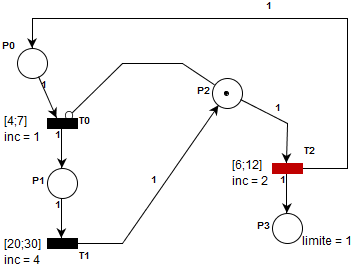
\includegraphics[keepaspectratio]{./desarrollo/diseno_implementacion/img/diseno35}
				\caption{Estado del procesador tras el proceso de carga (Red de Petri)}
				\label{fig:diseno35}
			\end{figure}
			\begin{figure}[H]
				\centering
				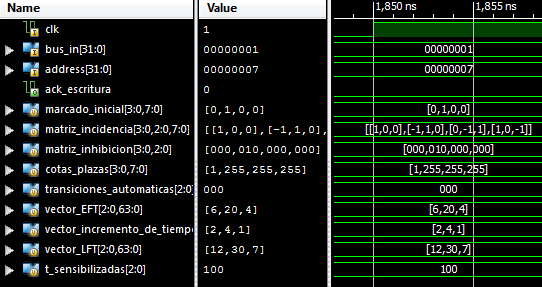
\includegraphics[width=0.8\linewidth,keepaspectratio]{./desarrollo/diseno_implementacion/img/diseno36}
				\caption{Estado del procesador tras el proceso de carga (Simulaci�n)}
				\label{fig:diseno36}
			\end{figure}
			
		\subsubsection{Secuencia de disparos}
		
			La secuencia de disparos elegida para probar este procesador ser�: 
			\begin{center}
				$S = { T0 , T2, T1 }$
			\end{center}
			
			\begin{enumerate}
			  	\item \emph{Solicitar el disparo de T0}
			  		
			  		Dado que al inicio la transici�n \emph{T0} no esta sensibilizada, solicitar 
			  		su disparo solo incrementar� la cola correspondiente.
			  		\begin{figure}[H]
						\centering
						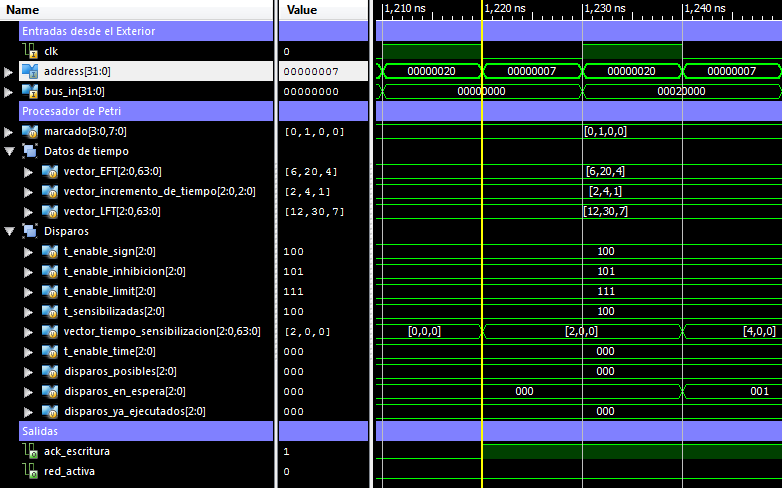
\includegraphics[width=0.8\linewidth,keepaspectratio]{./desarrollo/diseno_implementacion/img/diseno37}
						\caption{Solicitud de disparo de la transici�n \emph{T0} (simulaci�n)}
						\label{fig:diseno37}
					\end{figure}
			 		
			 	\newpage	
			 		
			  	\item \emph{Solicitar el disparo de T2}
			  		
			  		Como se observa en la Figura \ref{fig:diseno37} la solicitud de disparo de la transici�n 
			  		\emph{T2} llega inmediatamente despu�s de la solicitud de \emph{T0}. En ese instante, 
			  		la transici�n \emph{T2} se encuentra sensibilizada, pero, dadas las restricciones temporales, 
			  		no esta lista para dispararse. 
					\\
					
					En la Figura \ref{fig:diseno38}, se observa que desde el momento que \emph{T2} se sensibiliza,
					su marca de tiempo comienza a incrementarse en la cantidad de unidades indicada por el 
					\emph{vector de incrementos}. Al alcanzar el valor m�nimo indicado en el \emph{vector EFT} 
					ya es posible que se dispare.
					En el momento que la transici�n \emph{T2} es disparada, su marca de tiempo toma el valor cero.
					El disparo de la transici�n \emph{T2} deja la Red de Petri en un marcado que hace que la 
					transici�n \emph{T0} se sensibilice y quede sensibilizada. De esta manera, la marca de tiempo 
					de esta �ltima transici�n comienza a incrementarse. Y, como su disparo estaba en la cola de 
					espera, al llegar al \emph{valor EFT} correspondiente, se dispara.
					
			  		\begin{figure}[H]
						\centering
						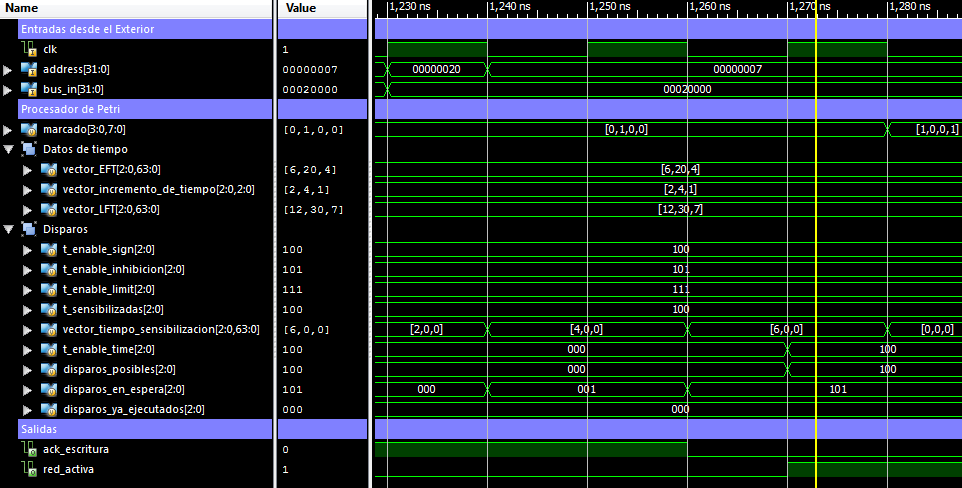
\includegraphics[width=1\linewidth,keepaspectratio]{./desarrollo/diseno_implementacion/img/diseno38}
						\caption{Solicitud y disparo de la transici�n \emph{T2}}
						\label{fig:diseno38}
					\end{figure}
					
					\newpage
					
					\begin{figure}[H]
						\centering
						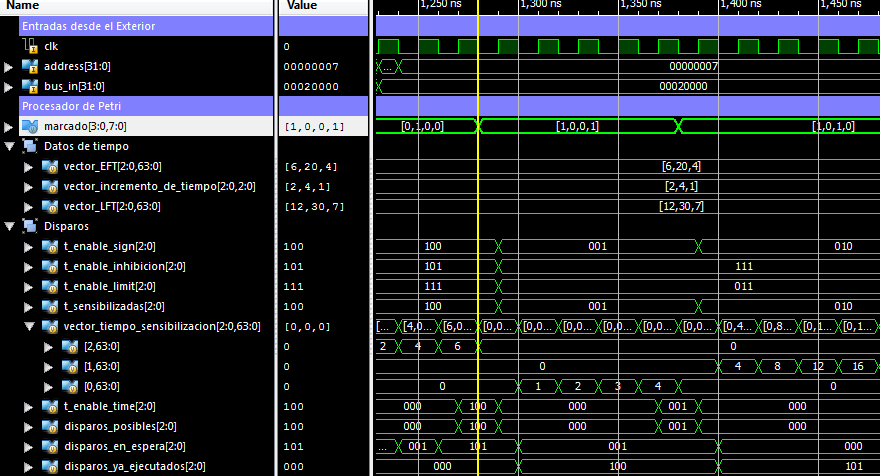
\includegraphics[width=1\linewidth,keepaspectratio]{./desarrollo/diseno_implementacion/img/diseno39}
						\caption{Disparo de la transici�n \emph{T0} (simulaci�n)}
						\label{fig:diseno39}
					\end{figure}
			  
			  	\item \emph{Solicitar el disparo de T1}
			  	
			  		Al dispararse la transici�n \emph{T0} resulta sensibilizada la transici�n \emph{T1} 
			  		y su marca de tiempo comienza a incrementarse. 
			  		\begin{figure}[H]
						\centering
						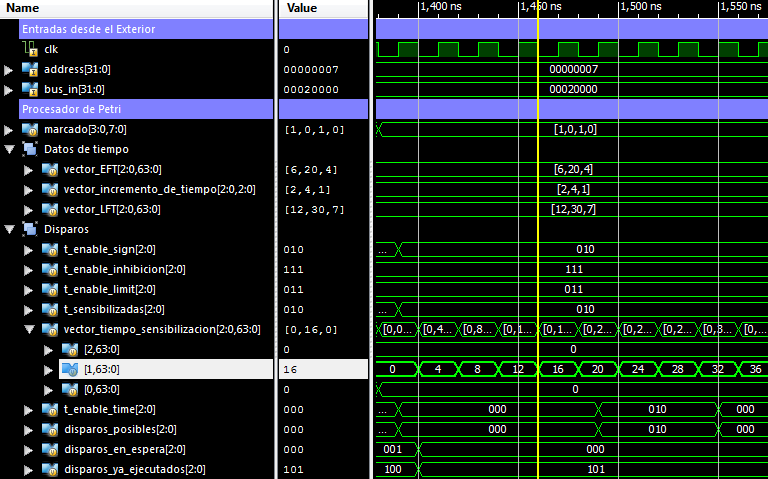
\includegraphics[width=0.95\linewidth,keepaspectratio]{./desarrollo/diseno_implementacion/img/diseno40}
						\caption{Habilitaci�n y des habilitaci�n de \emph{T1} (simulaci�n)}
						\label{fig:diseno40}
					\end{figure}
					Se debe recordar que la marca de tiempo de esta transici�n avanzaba de a cuatro unidades y 
					su intervalo de disparo es $[20;30]$.
					En la Figura \ref{fig:diseno40} se observa como, cuando la marca de tiempo de \emph{T1} se 
					sit�a dentro del intervalo, el disparo se hace posible, pero, la marca supera el \emph{valor LFT} 
					sin ser solicitado el disparo de la transici�n. De esta manera, al llegar la solicitud de 
					disparo \emph{T1} se almacena en la cola pero no puede ser ejecutado.
					\begin{figure}[H]
						\centering
						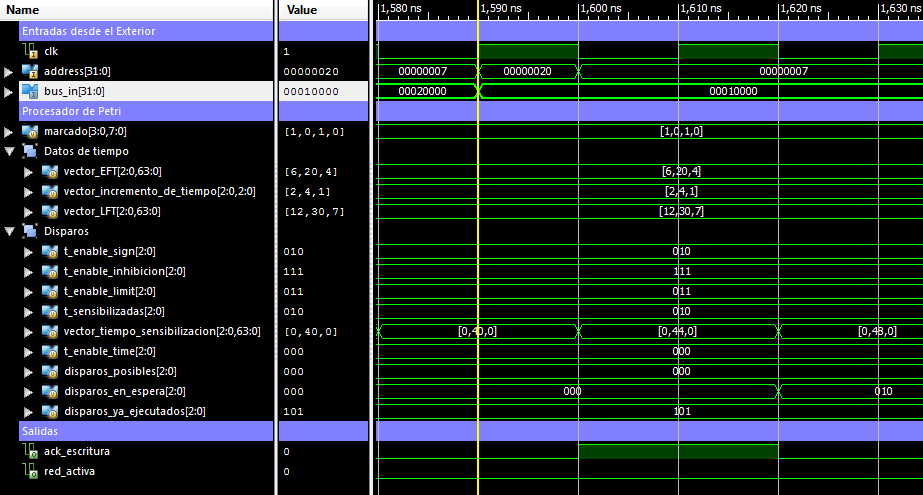
\includegraphics[width=0.95\linewidth,keepaspectratio]{./desarrollo/diseno_implementacion/img/diseno41}
						\caption{Habilitaci�n y des habilitaci�n de \emph{T1} (simulaci�n)}
						\label{fig:diseno41}
					\end{figure}
			  	
			\end{enumerate}			
	
		
	% Manejo de interrupciones
		%%%%%%%%%%%%%%%%%%%%%%%%%%%%%%%%%%%%%%%%%%%%%%%%%%%%%%%%%%%%%%%%%%%%%%%%%%%%%%%%%%%%%
%																					%
%	TRABAJO: Proyecto Integrador													%
%																					%
%		Titulo: 	Desarrollo de IP cores con procesamiento de Redes de Petri 		%
%					Temporales para sistemas multicore en FPGA						%
%																					%
%		Autores:	Juli�n Nonino													%
%					Carlos Renzo Pisetta											%
%		Director:	Orlando Micolini												%
%																					%
%	Parte: Desarrollo																%
%	Capitulo: Dise�o e Implementaci�n												%
%	Seccion: Manejo de interrupciones												%	
%	Archivo: manejo_interrupciones.tex												%
%																					%
%%%%%%%%%%%%%%%%%%%%%%%%%%%%%%%%%%%%%%%%%%%%%%%%%%%%%%%%%%%%%%%%%%%%%%%%%%%%%%%%%%%%%

% Path Imagenes: ./desarrollo/diseno_implementacion/img
% Nombre predeterminado imagenes: disenoxx
%	xx es el numero de imagen

\section{Manejo de interrupciones}
	\label{sec:manejo_interrupciones}

	Dado que ahora el procesador de Redes de Petri incluye el tiempo como una variable de ejecuci�n,
	puede ocurrir que una transici�n, luego de quedar sensibilizada requiera mucho tiempo antes de ser 
	ejecutada. En este caso, el proceso que solicite su disparo, el lugar de mantenerse activo esperando
	la ejecuci�n, podr�a suspenderse y que se reactive solo cuando la transici�n se haya ejecutado. Para 
	lograr esto, se implement� un sistema de interrupciones, cada vez que el procesador ejecuta un disparo
	interrumpe al sistema informando lo ocurrido. En �sta secci�n se detallar� como se ha desarrollado �sta
	funcionalidad.
	
	\subsection{Requerimientos}
	
		Para esta tercera etapa del trabajo, el requerimiento es agregarle al procesador de Redes de 
		Petri las conexiones y la l�gica necesaria para que genere interrupciones cada vez que un 
		disparo ha sido ejecutado.
		Adem�s se especificara un vector que enmascara las interrupciones de algunos disparos entonces, 
		el usuario puede decidir que disparos generaran interrupciones y cuales no.
		La idea que motiva esta tercera etapa es que como el procesador de Redes de Petri ahora considera 
		cuestiones temporales, ser�a deseable que los procesos/hilos tengan la posibilidad de suspenderse 
		en lugar de hacer una consulta permanente mientras esperan que su disparo sea ejecutado. De esta 
		manera, se liberan recursos del procesador y de la memoria.
		
	\subsection{Arquitectura}
		
		La arquitectura del procesador de Redes de Petri al incorporar el manejo de interrupciones se ve 
		afectada por el agregado de tres elementos.
		\begin{itemize}
		  	\item Un vector \textbf{\emph{Mascara de Interrupci�n}} cuyo objetivo es determinar cuales son 
		  		las transiciones que al dispararse generaran interrupciones.
		  	\item Un componente generador de interrupciones que contiene la l�gica encargada de determinar 
		  		en que momento generar la se�al la interrupci�n y de especificar como ser� dicha se�al.
		  	\item Un puerto f�sico por el cual enviar la se�al de interrupci�n.
		\end{itemize}
		Este m�dulo se encuentra conectado a un controlador de interrupciones del sistema, el \textbf{\emph{
		AXI Interrupt Controller}} \cite{xilinx_axi_int}.
		\begin{figure}[H]
			\centering
			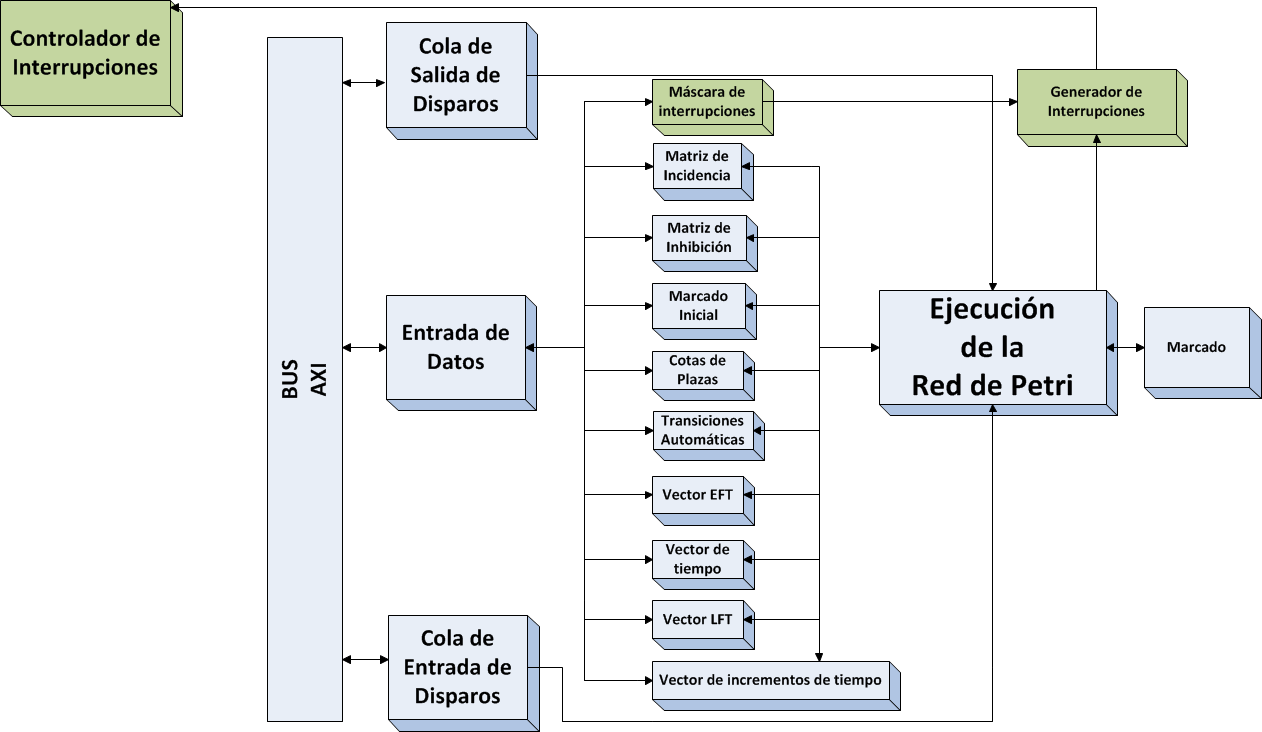
\includegraphics[width=1\linewidth,keepaspectratio]{./desarrollo/diseno_implementacion/img/diseno42}
			\caption{Arquitectura del Procesador de Redes de Petri con Interrupciones}
			\label{fig:diseno42}
		\end{figure}
		
		La Figura \ref{fig:diseno43} muestra un diagrama de componentes del m�dulo \emph{Generador de 
		Interrupciones}. La siguiente secci�n explicar� funcionamiento de este m�dulo y adem�s el 
		funcionamiento del sistema en su conjunto cuando el procesador de Redes de Petri tiene la 
		capacidad de interrumpir. 
			\begin{figure}[H]
				\centering
				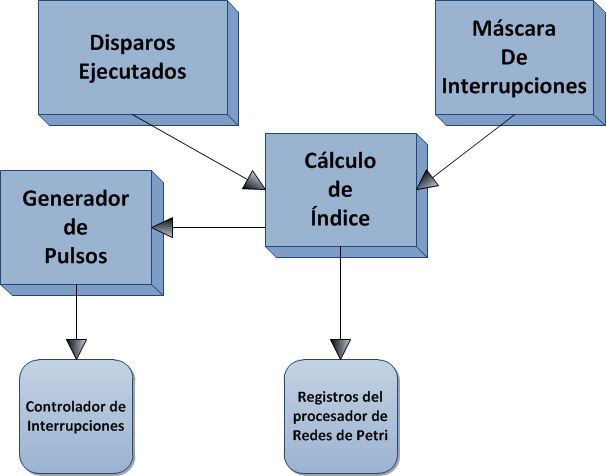
\includegraphics[width=0.75\linewidth,keepaspectratio]{./desarrollo/diseno_implementacion/img/diseno43}
				\caption{Diagrama de componentes del Generador de Interrupciones}
				\label{fig:diseno43}
			\end{figure}
					
	\subsection{Funcionamiento del sistema}
	
		B�sicamente, el generador de interrupciones, cada flanco negativo del reloj verifica si 
		alguno de las transiciones que est�n habilitadas para producir interrupciones se ha 
		ejecutado. Cuando esto sucede genera una se�al en \emph{1} de un ciclo de duraci�n. Adem�s, 
		determina el �ndice de dicha transici�n, para este procesador un valor entre cero (\emph{0}) y 
		doscientos cincuenta y cinco (\emph{255}).
		Dentro del sistema hardware/software el mecanismo de interrupci�n funciona tal como lo 
		muestra el diagrama de secuencia de la Figura \ref{fig:diseno44}.
		\\		

		Para limitar el n�mero de transiciones que al ser disparas generan una interrupci�n, se 
		utiliza el vector de m�scara de interrupciones que determina cuales transiciones interrumpen 
		y cuales no.
		Para que el disparo de una transici�n genere una interrupci�n el bit correspondiente en el 
		vector de m�scara de interrupciones debe estar en \emph{1} de lo contrario se dice que se 
		encuentra enmascarada no generar� interrupci�n alguna. Por lo tanto, para estas transiciones, 
		es tarea del usuario preguntar si ya ha sido ejecutada peri�dicamente o cuando lo crea necesario.
		
		El siguiente c�digo es Verilog es el encargado de generar el m�dulo encargado de las 
		interrupciones.
		
		\newpage
		
		\begin{lstlisting}
/*****GENERADOR DE INTERRUPCIONES*****/
reg [1:0]Interrupt_reg;
assign Interrupt=(!Interrupt_reg[1])&Interrupt_reg[0];

wire [cant_transiciones-1:0]intr_activadas;
assign intr_activadas=disparos_ya_ejecutados & intr_mask;

integer columnas_intr;

always@(negedge Bus2IP_Clk)
begin
	if (Bus2IP_Resetn==1'b0)
	begin
		num_intr<=0;
		Interrupt_reg<=2'b00;
	end
	else
	begin
		Interrupt_reg<={Interrupt_reg[0],(|(disparos_ya_ejecutados & intr_mask))&!intr_reset};//prioridad transicion menor
		for (columnas_intr=cant_transiciones-1 ; columnas_intr>=0 ; columnas_intr=columnas_intr-1)
		begin
			if(intr_activadas[columnas_intr]==1'b1)	num_intr<=columnas_intr;
		end
	end
end
\end{lstlisting}
		
		\begin{figure}[H]
			\centering
			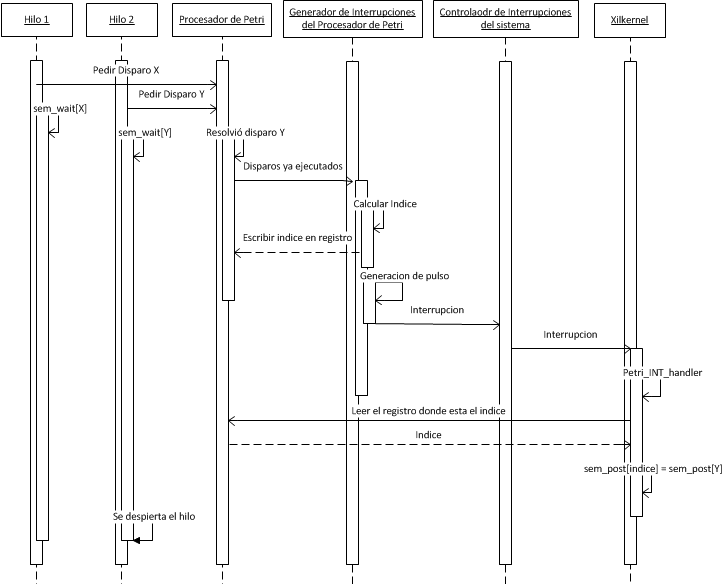
\includegraphics[width=0.9\linewidth,keepaspectratio]{./desarrollo/diseno_implementacion/img/diseno44}
			\caption{Diagrama de secuencia del proceso de generaci�n y atenci�n de una interrupci�n}
			\label{fig:diseno44}
		\end{figure}
		
	\subsection{Verificaci�n}
		
		Para la verificaci�n del funcionamiento de las interrupciones del procesador de Redes de Petri se 
		utilizar� la red de la Figura \ref{fig:diseno45}.	
		\begin{figure}[H]
			\centering
			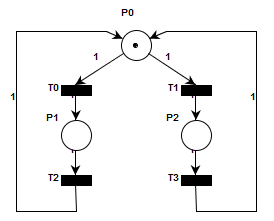
\includegraphics[width=0.4\linewidth,keepaspectratio]{./desarrollo/diseno_implementacion/img/diseno45}
			\caption{Red de Petri para la verificaci�n del funcionamiento de las interrupciones}
			\label{fig:diseno45}
		\end{figure}
		
		\begin{center}
			\begin{tabular}{c c c}
				% Primera Fila
					% Columna Uno
						$m_0 = \begin{bmatrix}
						  				1 \\
						  				0 \\
  						  				0
  									\end{bmatrix}$ 
  						& 
  						% Columna dos
  							$I = \begin{bmatrix}
						  				-1 	& 1	& 1		& 1		\\
						  				1 	& 0	& -1	& 0		\\
  						  				0 	& 1 & 0		& -1
  						  		\end{bmatrix}$  
  						&
  						%Columna Tres
  							$H = \begin{bmatrix}
						  				0 & 0 & 0 & 0 \\
						  				0 & 0 & 0 & 0 \\
  						  				0 & 0 & 0 & 0
  						  		\end{bmatrix}$    
				\\
				%Segunda Fila
					\emph{Marcado Inicial} & \emph{Matriz de Incidencia} & \emph{Matriz de Inhibici�n} 				
				\end{tabular}
		\end{center}
		
		\begin{center}
			\begin{tabular}{c c}
				% Primera Fila
					% Columna Uno
						$\begin{bmatrix}
						  				P_0 \\
						  				P_1 \\
  						  				P_2 
  							\end{bmatrix} 
  							= 
  							\begin{bmatrix}
						  		max \\
						  		max \\
  						  		max
  							\end{bmatrix}$ 
  						& 
  						% Columna dos
						$\begin{bmatrix}
						  				T_0 \\
						  				T_1 \\
  						  				T_2 \\
  						  				T_3
  							\end{bmatrix} 
  							= 
  							\begin{bmatrix}
						  		0 \\
						  		0 \\
  						  		0 \\
  						  		0
  							\end{bmatrix}$
				\\
				%Segunda Fila
					\emph{Vector de Cotas de Plazas} & \emph{Vector de Transiciones Autom�ticas}				
				\end{tabular}
		\end{center}
		
		\begin{center}
			\begin{tabular}{c c c}
				% Primera Fila
					% Columna Uno
						$\begin{bmatrix}
						  				T_0 \\
						  				T_1 \\
  						  				T_2 \\
  						  				T_3
  							\end{bmatrix} 
  							= 
  							\begin{bmatrix}
						  		0 \\
						  		0 \\
  						  		0 \\
  						  		0
  							\end{bmatrix}$ 
  						& 
  						% Columna dos
						$\begin{bmatrix}
						  				T_0 \\
						  				T_1 \\
  						  				T_2 \\
  						  				T_3
  							\end{bmatrix} 
  							= 
  							\begin{bmatrix}
						  		1 \\
						  		1 \\
  						  		1 \\
  						  		1
  							\end{bmatrix}$ 
  						&
  						%Columna Tres
						$\begin{bmatrix}
						  		T_0 \\
						  		T_1 \\
  						  		T_2 \\
  						  		T_3 
  							\end{bmatrix} 
  							= 
  							\begin{bmatrix}
						  		max \\
						  		max \\
  						  		max \\
  						  		max
  							\end{bmatrix}$ 
				\\
				%Segunda Fila
					\emph{Vector EFT} & \emph{Vector de Incrementos de Tiempo} & \emph{Vector LFT} 				
				\end{tabular}
		\end{center}
		
		\begin{center}
			\begin{tabular}{c}
	   			$\begin{bmatrix}
						T_0 \\
						T_1 \\
  						T_2 \\
  						T_3
  					\end{bmatrix} 
  					= 
  					\begin{bmatrix}
						0 \\
						1 \\
  						1 \\
  						0
  					\end{bmatrix}$ 	 
				\\
				\emph{Vector de M�scara de Interrupciones}
			\end{tabular}
		\end{center}
			
		Donde se destaca el \textbf{\emph{Vector de Mascara de Interrupciones}} que indica que 
		transiciones son las que pueden generar interrupciones. En este caso, solo las transiciones
		\emph{T1} y \emph{T2}.
		\\
		
		Se escribi� un test en Verilog para verificar el funcionamiento del procesador de Redes de 
		Petri, solicitando la ejecuci�n de las transiciones \emph{T0} y \emph{T2}.
		Los resultados de la simulaci�n se presentan en las im�genes a continuaci�n.
		\begin{figure}[H]
			\centering
			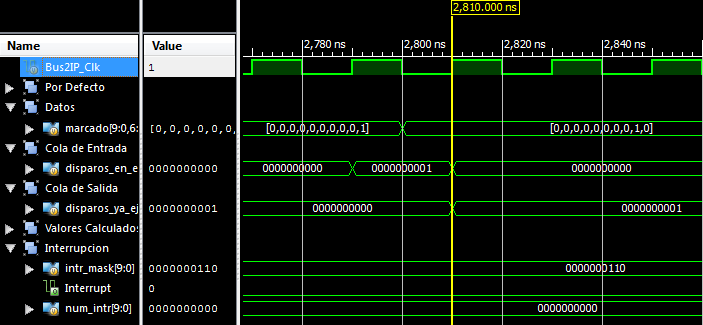
\includegraphics[width=0.85\linewidth,keepaspectratio]{./desarrollo/diseno_implementacion/img/diseno46}
			\caption{Simulaci�n del disparo de \emph{T0} (NO interrumpe)}
			\label{fig:diseno46}
		\end{figure}
			
		En la simulaci�n de la Figura \ref{fig:diseno46} se observa que el disparo \emph{T0} est� 
		en la cola de entrada. Luego, al ejecutarse, actualiza el marcada y pasa a la cola de salida,
		pero debido a la mascara de interrupciones (vector \emph{intr mask}) no genera interrupci�n.
		
		\begin{figure}[H]
			\centering
			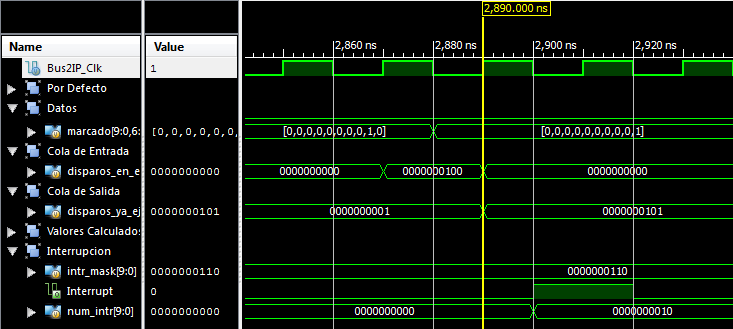
\includegraphics[width=0.85\linewidth,keepaspectratio]{./desarrollo/diseno_implementacion/img/diseno47}
			\caption{Simulaci�n del disparo de \emph{T2} (SI interrumpe)}
			\label{fig:diseno47}
		\end{figure}
		
		En la Figura \ref{fig:diseno47} se observa a \emph{T2} en la cola de espera. Luego, en el flaco 
		positivo del \emph{Bus2IP Clk} a los 2890 ns el disparo es ejecutado y pasa a la cola de salida. 
		Medio ciclo mas tarde se produce un pulso de interrupci�n que dura un ciclo exactamente. Esto se 
		debe a que el disparo de \emph{T2} no estaba enmascarado.
		
	
	% IP core para Redes de Petri Temporizadas
		%%%%%%%%%%%%%%%%%%%%%%%%%%%%%%%%%%%%%%%%%%%%%%%%%%%%%%%%%%%%%%%%%%%%%%%%%%%%%%%%%%%%%
%																					%
%	TRABAJO: Proyecto Integrador													%
%																					%
%		Titulo: 	Desarrollo de IP cores con procesamiento de Redes de Petri 		%
%					Temporales para sistemas multicore en FPGA						%
%																					%
%		Autores:	Juli�n Nonino													%
%					Carlos Renzo Pisetta											%
%		Director:	Orlando Micolini												%
%																					%
%	Parte: Desarrollo																%
%	Capitulo: Dise�o e Implementaci�n												%
%	Seccion: IP core para Redes de Petri Temporizadas								%	
%	Archivo: redes_temporizadas.tex													%
%																					%
%%%%%%%%%%%%%%%%%%%%%%%%%%%%%%%%%%%%%%%%%%%%%%%%%%%%%%%%%%%%%%%%%%%%%%%%%%%%%%%%%%%%%

% Path Imagenes: ./desarrollo/diseno_implementacion/img
% Nombre predeterminado imagenes: disenoxx
%	xx es el numero de imagen

\section{IP core para Redes de Petri Temporizadas}
	\label{sec:redes_temporizadas}

	Como se mencion� en los objetivos de este trabajo, se generar�n IP cores para las dos sem�nticas
	de tiempo existentes. En las secciones anteriores, se trabaj� con la sem�ntica de las \emph{Redes de
	Petri con Tiempo}. En este apartado, se detallar� el dise�o y la implementaci�n del Ip core que procesar�
	\textbf{\emph{Redes de Petri Temporizadas}} manteniendo la capacidad de generar interrupciones.
	
	\subsection{Requerimientos}
	
		En esta �ltima etapa, el requerimiento es realizar las modificaciones necesarias sobre el IP core 
		generado en las etapas anteriores para lograr un nuevo IP core que sea capaz de resolver Redes de 
		Petri Temporizadas.
	
	\subsection{Arquitectura}
	
		La arquitectura de este IP core se mantiene en su mayor parte igual a la de las versiones anteriores. 
		Con respecto a la versi�n que procesa \emph{Redes de Petri con Tiempo}, se quitaron los vectores \emph{EFT} 
		y \emph{LFT}, en su lugar se agreg� el \textbf{\emph{vector duraci�n}}. Se mantuvo el \textbf{\emph{vector de 
		incrementos de tiempo}} y el \textbf{\emph{vector de tiempo de sensibilizaci�n}}.
			
			\begin{figure}[H]
				\centering
				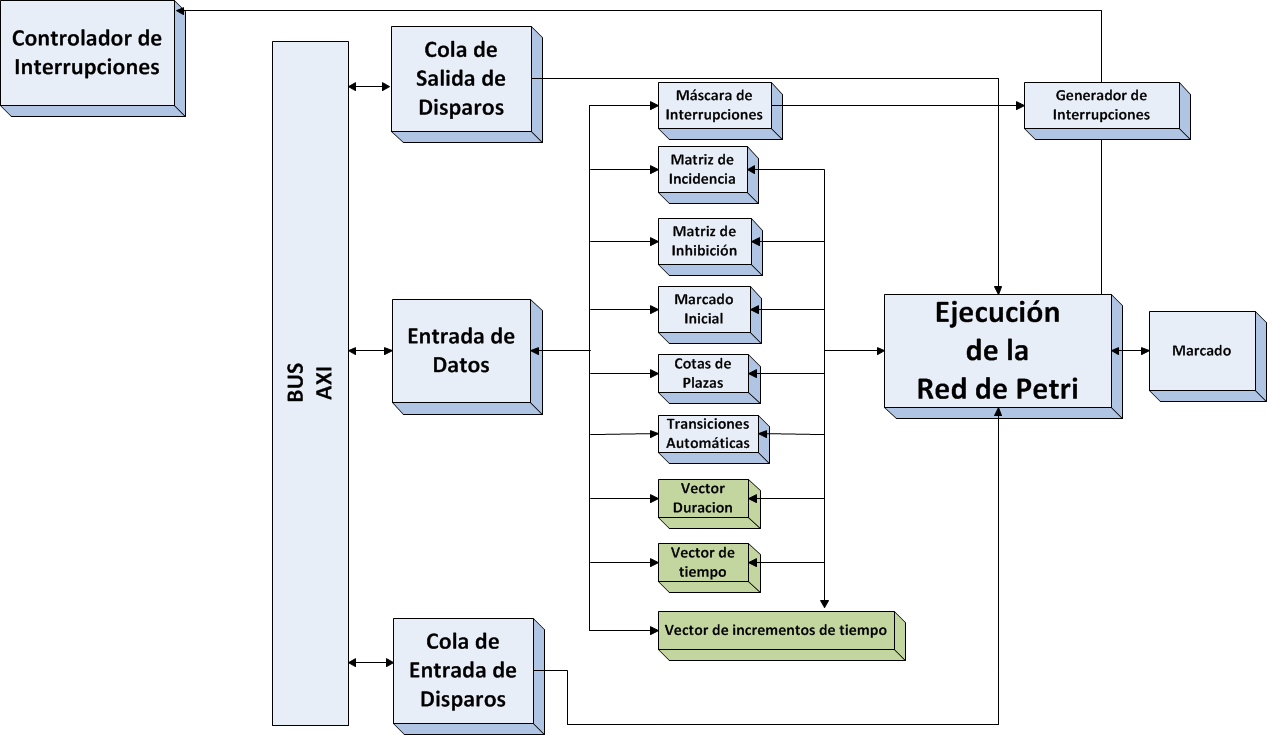
\includegraphics[width=1\linewidth,keepaspectratio]{./desarrollo/diseno_implementacion/img/diseno48}
				\caption{Arquitectura del procesador de Redes de Petri Temporizadas}
				\label{fig:diseno48}
			\end{figure}
		
	\subsection{Estructuras de datos para Redes de Petri Temporizadas}
	
		Como se muestra en la Figura \ref{fig:diseno48} las estructuras de datos necesarias para la resoluci�n 
		de Redes de Petri Temporizadas son tres:
		\begin{itemize}
		  	\item Vector \textbf{\emph{duraci�n}}.
		  	\item Vector de \textbf{\emph{marcas temporales}}.
		  	\item Vector de \textbf{\emph{escala de incrementos de tiempo}}.
		\end{itemize}
		
		Los cuatro vectores tienen como cantidad de elementos el n�mero de transiciones. Los dos primeros son 
		tiene un tama�o de elementos parametrizable pero por defecto tienen 32 bits. El vector de escala de 
		incrementos de tiempo, por defecto toma el un tama�o de elementos de 5 bits.
		
	\subsection{Determinaci�n de disparos posibles}
	
		Para que un disparo sea posible en una Red de Petri, debe cumplir las condiciones dadas por que todas 
		las transiciones de las cuales toma tokens tengan la cantidad necesaria de tokens, que las plazas a las 
		cuales esta conectada con arcos inhibidores no tengan tokens y que las plazas en las cuales depositan 
		tokens no superen los limites impuestos por las cotas en las plazas.
		En una Red de Petri Temporizada, al cumplirse las condiciones antes mencionadas, se dice que la transici�n 
		esta \textbf{\emph{sensibilizada}}, entonces, se ejecuta la ecuaci�n de estado de la Red de Petri utilizando 
		la matriz $I^-$. De esta manera, se remueven todos los tokens de las plazas de entrada.
			
			\begin{equation}
				m_{i+1} = m_i + I^+ � \delta
			\end{equation}

		D�nde $\delta$ es el vector de disparo que se desea ejecutar.
		A partir de dicho momento, la marca de tiempo asociada a la transici�n comienza a incrementarse seg�n su 
		vector de incrementos de tiempo. Cuando esta marca de tiempo alcanza el valor indicado por el \textbf{\emph{
		vector duraci�n}}. Cuando esto ocurre, el disparo ya esta habilitado para ser ejecutado completamente. 
		Esto se hace ejecutando la ecuaci�n de estado con la matriz de incidencia positiva, esto implica poner los tokens en 
		todas las plazas de salida.
		
			\begin{equation}
				m_{i+1} = m_i + I^- � \delta
			\end{equation}

		Durante el proceso de carga y en el instante en el cual este termina, las marcas de tiempo de todas las 
		transiciones valen cero. 
		Luego, a cada ciclo de reloj, si la transici�n se sensibiliz� y logo ejecutar la primera etapa del disparo, 
		la marca de tiempo se incrementa la cantidad de unidades que indica el \textbf{\emph{vector de incrementos de marcas 
		de tiempo}}.
		La marca de tiempo vuelve a cero solo cuando la transici�n completa ambas fases de su disparo.
			
	\subsection{Verificaci�n}
		
		Para la verificaci�n del funcionamiento del procesador de Redes de Petri Temporizadas, se utilizar� la 
		siguiente red:
			\begin{figure}[H]
				\centering
				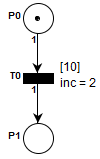
\includegraphics[width=0.2\linewidth,keepaspectratio]{./desarrollo/diseno_implementacion/img/diseno49}
				\caption{Red de Petri para la verificaci�n del procesador de Redes de Petri Temporizadas}
				\label{fig:diseno49}
			\end{figure}
			
		Los datos correspondientes a �sta Red de Petri Temporizada son:
			
			\begin{center}
				\begin{tabular}{c c}
					% Primera Fila
						% Columna Uno
							$m_0 = \begin{bmatrix}
 						  				1 \\
 						  				0
   									\end{bmatrix}$ 
   						&
   						% Columna dos
							$\begin{bmatrix}
 						  				P_0 \\
 						  				P_1
   							\end{bmatrix} 
   							= 
   							\begin{bmatrix}
 						  		max \\
 						  		max
   							\end{bmatrix}$  
					\\
					%Segunda Fila
						\emph{Marcado Inicial} & \emph{Vector de Cotas de Plazas} 				
					\end{tabular}
			\end{center}

			\begin{center}
				\begin{tabular}{c c}
					% Primera Fila
						% Columna uno
   							$I^+ = \begin{bmatrix}
 						  				0 \\
 						  				1
   						  		\end{bmatrix}$  
   						&
   						% Columna dos
   						$I^- = \begin{bmatrix}
 						  				1 \\
 						  				0
   						  		\end{bmatrix}$ 
					\\
					%Segunda Fila
						\emph{Matriz de Incidencia Positiva} & \emph{Matriz de Incidencia Negativa}	
					\end{tabular}
			\end{center}

			\begin{center}
				\begin{tabular}{c c}
					% Primera Fila
						%Columna uno
   							$H = \begin{bmatrix}
 						  				0 \\
 						  				0
   						  		\end{bmatrix}$ 
   						& 
   						% Columna dos
							$\begin{bmatrix}
 						  				T_0
   							\end{bmatrix} 
   							= 
   							\begin{bmatrix}
 						  		0
   							\end{bmatrix}$
					\\
					%Segunda Fila
						\emph{matriz de Inhibici�n} & \emph{Vector de Transiciones Autom�ticas}				
					\end{tabular}
			\end{center}

			\begin{center}
				\begin{tabular}{c c}
					% Primera Fila
						% Columna Uno
							$\begin{bmatrix}
 						  				T_0
   							\end{bmatrix} 
   							= 
   							\begin{bmatrix}
 						  		10
   							\end{bmatrix}$ 
   						& 
   						% Columna dos
							$\begin{bmatrix}
 						  				T_0
   							\end{bmatrix} 
   							= 
   							\begin{bmatrix}
 						  		2
   							\end{bmatrix}$ 		
					\\
					%Segunda Fila
						\emph{Vector duraci�n} & \emph{Vector de Incrementos de Tiempo} 				
					\end{tabular}
			\end{center}

			\begin{center}
				\begin{tabular}{c}
		   			$\begin{bmatrix}
 						T_0
   					\end{bmatrix} 
   					= 
   					\begin{bmatrix}
 						1
   					\end{bmatrix}$  
					\\
					\emph{Vector de M�scara de Interrupciones}
				\end{tabular}
			\end{center}
		
		La Figura \ref{fig:diseno50}, muestra todos los datos mencionados anteriormente cargados dentro del procesador de 
		Redes de Petri.
		
			\begin{figure}[H]
				\centering
				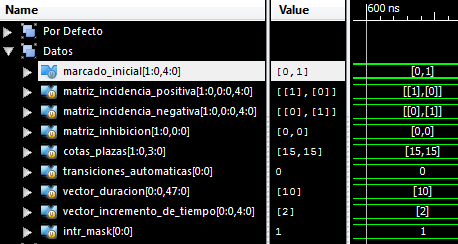
\includegraphics[keepaspectratio]{./desarrollo/diseno_implementacion/img/diseno50}
				\caption{Valores cargados dentro del procesador de Redes de Petri Temporizadas}
				\label{fig:diseno50}
			\end{figure}
		
		Luego de la carga de datos, la Figura \ref{fig:diseno51} muestra el estado del procesador.	
			
			\begin{figure}[H]
				\centering
				\includegraphics[width=0.8\linewidth,keepaspectratio]{./desarrollo/diseno_implementacion/img/diseno51}
				\caption{Estado del procesador de Redes de Petri Temporizadas luego de la carga de datos}
				\label{fig:diseno51}
			\end{figure}
			
		A continuaci�n se solicita el disparo de la transici�n \emph{T0} y se analizar� paso a pasos desde 
		la solicitud del disparo, las dos fases de ejecuci�n y la aparici�n en el vector de disparos ya 
		ejecutados.
			
			\begin{figure}[H]
				\centering
				\includegraphics[width=0.8\linewidth,keepaspectratio]{./desarrollo/diseno_implementacion/img/diseno52}
				\caption{Llegada de la solicitud de disparo \emph{T0} y ejecuci�n}
				\label{fig:diseno52}
			\end{figure}
			
		La Figura \ref{fig:diseno52} muestra la llegada de la solicitud del disparo de la transici�n \emph{T0}, 
		como ingresa a la cola de entrada, las dos fases de ejecuci�n y como se lo incluye en la cola de disparos 
		ya ejecutados.
		
		La l�nea amarilla marca el instante en el cual la solicitud de disparo es introducida en la cola de 
		entrada de disparos. Dado que esa transici�n estaba sensibilizada, en el flanco negativo siguiente, 
		es realizada la primera fase de la ejecuci�n, se extraen los tokens de la plaza de entrada (en este caso, 
		sacar un token \emph{P0}). Tambi�n, el disparo es retirado de la cola de entrada y en el vector 
		\emph{mask semi ejecucion}, la transici�n es marcada como que esta ejecut�ndose y no podr� ser disparada 
		nuevamente.

		A partir de dicho instante, el vector de marca de tiempo (\emph{vector tiempo sensibilizacion}) comienza 
		a incrementarse a cada ciclo de reloj seg�n como lo indica el vector de incrementos de tiempo.

		Cuando el vector de marcas de tiempo es igual o mayor al valor indicado en el vector de duraci�n, se 
		inicia la segunda fase ejecuci�n. Esta fase consiste en colocar los tokens necesarios en todas las plazas 
		de salida de la transici�n (en este caso, colocar un token en \emph{P1}). Luego, se pone un \emph{1}
		otra vez en el vector \emph{mask semi ejecucion}, haciendo que la transici�n vuelva a estar disponible 
		para ser disparada. 
	 
		Por �ltimo, el disparo es cargado en la cola de disparos ya ejecutados.
		
							